\chapter{Kerne- og Partikelfysik}
\section{Kernefysik}
I centrum af ethvert atom befinder sig en utrolig tæt, positivt ladet kerne. Atomets udstrækning er af størrelsesordenen $10^{-10}$ m, mens selve kernen kun udspænder cirka $10^{-15}$ m -- kernen er derfor 100.000 gange mindre end atomet. Alligevel befinder størstedelen af atomets masse sig i kernen. Atomkernen udgøres af postitive partikler \textit{protoner} (skrevet som ''p'') og neutrale partikler \textit{neutroner} (skrevet som ''n''). Kernen holdes sammen af den stærke kernekraft, én af de fire fundamentale kræfter. Denne kraft konkurrerer med den elektriske frastødning, som protonerne udøver på hinanden, og dette afgør, om kernen er stabil eller ustabil. Ustabile kerne kan henfalde - omdanne sig selv til en anden sammensætning ved en række processer. 
Dette afsnit vil give et kort overblik over kernefysikken - kategoriseringen af kernerne, hvilke modeller der kan bruges til at beskrive deres egenskaber og hvordan de kan gennemgå henfald. 

\subsection{Kernernes Egenskaber}
Eksperimentelt set har det vist sig, at atomets kerne kan ses som en kugle med radius $R$ indeholdene et antal \textit{nukleoner} - protoner og neutroner. Dette antal skrives som $A$. 
For de fleste kerner gælder det, at kernens radius kan udtrykkes som 
\begin{equation}
R = R_0A^{1/3},
\end{equation}
hvor $R_0$ er en eksperimentel konstant:
\begin{equation}
R_0 = 1,2\cdot {10^{-15}} ~ \SI{}{\m} = 1,2 ~\SI{}{\femto\m}. \footnotemark
\end{equation}

\footnotetext{ Her står ''fm'' for \emph{femto}-meter, hvor $\text{femto}=10^{-15}$}

\begin{table}
    \begin{tabular}{l|l|l|l}
    Partikel            & Masse, [kg]                      & Masse, [u]                       & Masse, [MeV/$\text{c}^2$] \\ \hline
    1 atomar masseenhed & 9,109 382 91 $\cdot 10^{-31}$   & 1                                & 931,494 061               \\
    Neutron             & 1,674 927 351 $\cdot 10^{-27} $ & 1,008 664 916 00                 & 939, 565 379              \\
    Proton              & 1,672 621 777 $\cdot 10^{-27}$  & 1,007 276 466 812                & 938, 272 046              \\
    Elektron            & 9,19 382 91 $\cdot 10^{-31}$    & 5,485 799 0946  $\cdot 10^{-4}$ & 0,510 998 928             \\
    \end{tabular}
    \caption{Massen af den atomare masseenhed, neutronen, protonen og elektronen i udvalgte enheder}
    \label{tab:masser}
\end{table}

Nukleon-tallet $A$ kaldes også for \emph{massetallet}, idet det lægger sig tæt op ad kernens masse udtrykt i \emph{atomare masseenheder}. Én atomar masseenhed, skrevet u eller $m_u$, er af historiske årsager defineret som en tolvtedel af massen af Carbon-12:

\begin{equation}
\text{u} = m_u \equiv \frac{1}{12} M(^{12}\text{C}).
\label{eq:u}
\end{equation} 

Tabel \ref{tab:masser} viser massen af den atomare masseenhed, samt neutronen, protonen og elektronen i enheder af henholdsvis kg, u og $\text{MeV}/\text{c}^2$ \footnotemark .

\footnotetext{Enheden $\text{MeV}/\text{c}^2$ er mega ($10^6$) elektronvolt over kvadratet af lysets hastighed $c$. Masse og energi er direkte koblet gennem Einsteins formel $E=mc^2$, ud fra det følger at en masse kan skrives som $m=E/c^2$.}

Det ses, hvordan protonens og neutronens masser er meget tæt på 1 u, og det er derfor $A$ tilnærmelsesvist giver massen af kernen i atomare masseenheder.

Som sagt er kernens massetal, $A$, antallet af nukleoner i kernen, altså summen af kernens antal protoner (skrevet som $Z$) og neutroner (skrevet som $N$):

\begin{equation}
A = Z + N.
\label{eq:A}
\end{equation}  

Kernens grundstof, også nogle gange kaldet kernens element, er bestemt af antal protoner, $Z$. For eksempel har hydrogen (H) altid én proton, helium (He) har to, og uran (U) har 92.
Kerner af det samme grundstof kan dog have forskellig masse ($A$) ved at have forskellige antal neutroner, $N$. Kerner med samme $Z$, men forskellig $N$ kaldes \emph{isotoper}. Tages uran ($Z=92$) som eksempel, er to almindeligt forekommende isotoper Uran--235 (massetal $A=235$ og $N=A-Z=143$) og Uran--238 ($N=146$). I fysikken kan vi bruge forskellig notation til at angive et grundstof på forskellige måder. Ser vi igen på Uran, kan vi angive hvilken isotop, der er tale om, ved at skrive "Uran--235", "U--235" eller 
\begin{equation*}
^{235}_{~92}\text{U}_{143}.
\end{equation*}

Her ses det, at notationen for et vilkårligt grundstof X følger:
\begin{equation*}
^{A}_{Z}\text{X}_{N},
\end{equation*}

men man vil oftest udelade informationen om $Z$ og $N$, idet grundstoffet selv er defineret ud fra $Z$, og $N$ opnås som $N=A-Z$. Man skriver derfor

\begin{equation}
^{A}\text{X}.
\end{equation}

\subsection{Kerners Binding}
I en kerne er nukleonerne samlet indenfor et begrænset område -- man siger, at kernen er et \emph{bundent system} \footnotemark .

\footnotetext{ En mere "fysisk" beskrivelse ville lyde på, at en partikel i et bundent system er udsat for et \emph{potential}, som kan holde partiklen lokaliseret. Potentialet kan være en ydre påvirkning (som et kraftfelt) eller kan være opstået som resultat af vekselvirkningen mellem det bundne systems komponenter. }

En vigtig egenskab for kernerne kan belyses gennem et simpelt eksempel. En alfa-partikel er et bundent system, bestående af to protoner og to neutroner (identisk til en helium--kerne). Massen af alfa-partikler i atomare masseenheder er målt til at være 4.001506179125 u. Den samlede masse af de to protoner og to neutroner kan udregnes til:

\begin{align*}
N \cdot m_n + Z \cdot m_p &= 2 \cdot 1,008 664 916 00~\SI{}{u} + 2 \cdot 1,007 276 466 812~\SI{}{u} \\
&= 4,031 88276562~\SI{}{u}.
\end{align*}  

Dette er ikke tilsvarende massen af alfa-partiklen! Faktisk ser vi, hvordan alfa-partiklen, det bundne system, har \emph{mindre} masse end summen af masserne for de tilstedeværende protoner og neutroner! Dette er tilfældet for alle kerners masse sammenlignet med massen af de individuelle nukleoner. Dette skyldes, at det bunde system har mindre \emph{potentiel energi}, end hvad de individuelle nukleoner oplever. Simpelt sagt kan man sige, at noget af massen "forsvinder" og bliver lagret i form af energi, når individuelle nukleoner bliver bundet sammen i kerner.

Forskellen i masse mellem kernen og massesummen af nukleonerne kaldes for \emph{massedefekten}, skrevet som $\Delta M$ (udtales "delta-M"):

\begin{equation}
\Delta M \equiv M(Z,A) - Z (m_p + m_e) - N \cdot m_n.
\label{eq:mass_excess}
\end{equation}

Læg mærke til, at massen $m_e$ -- elektronens masse -- optræder i formlen. Dette skyldes at $M(Z,A)$ er den \emph{atomare masse} af elementet, massen af kernen medtaget elektronerne om kernen. Et "uændret" atom er neutralt, og har derfor lige mange protoner og elektroner, derfor ganges $m_e$ med antallet af protoner $Z$.
 
Vi kan vende tilbage til vores eksempel med alfa-partiklen og udregne massedefekten. I dette tilfælde har vi massen $M_\alpha$ af alfa-partiklen opgivet ($M(2,4)$, uden bidraget fra elektronerne), svarende til størrelsen $M_\alpha=M(2,4)-2\times m_e$. Massedefekten udregnes da som:

\begin{align*}
\Delta M &= M_\alpha + 2\cdot m_e - Z(m_p + m_e) - N \cdot m_n \\
&= M_\alpha - Z \cdot m_p - N \cdot m_n \\
&= 4,001506179125~\SI{}{u} - 2 \cdot 1,008 664 916 00~\SI{}{u} - 2 \cdot 1,007 276 466 812~\SI{}{u} \\
&= -0,03037658649~\SI{}{u}
\end{align*}

Dette er altså forskellen mellem massen af alfa-partiklen og massen af de to protoner og to neutroner. Masse og energi er ækvivalente gennem Einsteins formel

\begin{equation}
E = m c^2, 
\label{eq:einstein}
\end{equation}

hvor $c$ er lysets hastighed.
Så hvad svarer den manglende masse til i energi? Læg her mærke til, at den atomare masseenhed u også kan udtrykkes i den meget praktiske enhed $\text{MeV}/c^2$, hvor $1~\SI{}{u}=931,494061~\SI{}{MeV}/c^2$. Derfor kan vi direkte omregne massedefekten til energi:

\begin{align*}
E &= \Delta M c^2 \cdot 931,494061~\SI{}{MeV}/c^2/\SI{}{u} \\
&= -0,03037658649 ~\SI{}{u} c^2 \cdot 931,494061~\SI{}{MeV}/c^2/\SI{}{u} \\
&= -28,2956099089 ~\SI{}{MeV}
\end{align*}

Denne størrelse -- uden fortegnet! -- er kernens \emph{bindingsenergi}. Bindingsenergien er den energi, som skal tilføres det bundne system for at skille det ad til dets individuelle nukleoner. Jo større bindingsenergi, desto sværere er det at skille kernen ad, sagt med andre ord, at jo højere bindingsenergi, desto mere stabil er kernen. Omvendt er bindingsenergien den energi der udløses, ved at samle frie nukleoner --  eller kerner -- til større systemer. Dette er princippet bag \emph{fusion}, den sammensmeltning af mindre elementer til tungere elementer, som foregår i Solen og andre stjerner for at producere energi.
Bindingsenergi, skrevet $E_B$ udtrykkes altid som en positiv størrelse. Udtrykt som funktion af massedefekten kan vi derfor skrive:
\begin{equation}
E_B = - \Delta M c^2.
\label{eq:binding}
\end{equation} 

En kernes bindingsenergi vil ændre sig, hvis der tilføjes eller fjernes nukleoner fra kernen, og \emph{vil altid stige med antallet af nukleoner, $A$}. Selvom nukleonerne i sig selv ikke besidder bindingsenergi, kan vi forestille os, at bindingsenergien for en kerne kan deles ligeligt mellem dens nukleoner. Denne størrelse kaldes for (den gennemsnitlige) bindingsenergi per nukleon, $E_B/A$. Figur \ref{fig:binding} viser $E_B/A$ som funktion af $A$. 

\begin{figure}[h]!
  \centering
  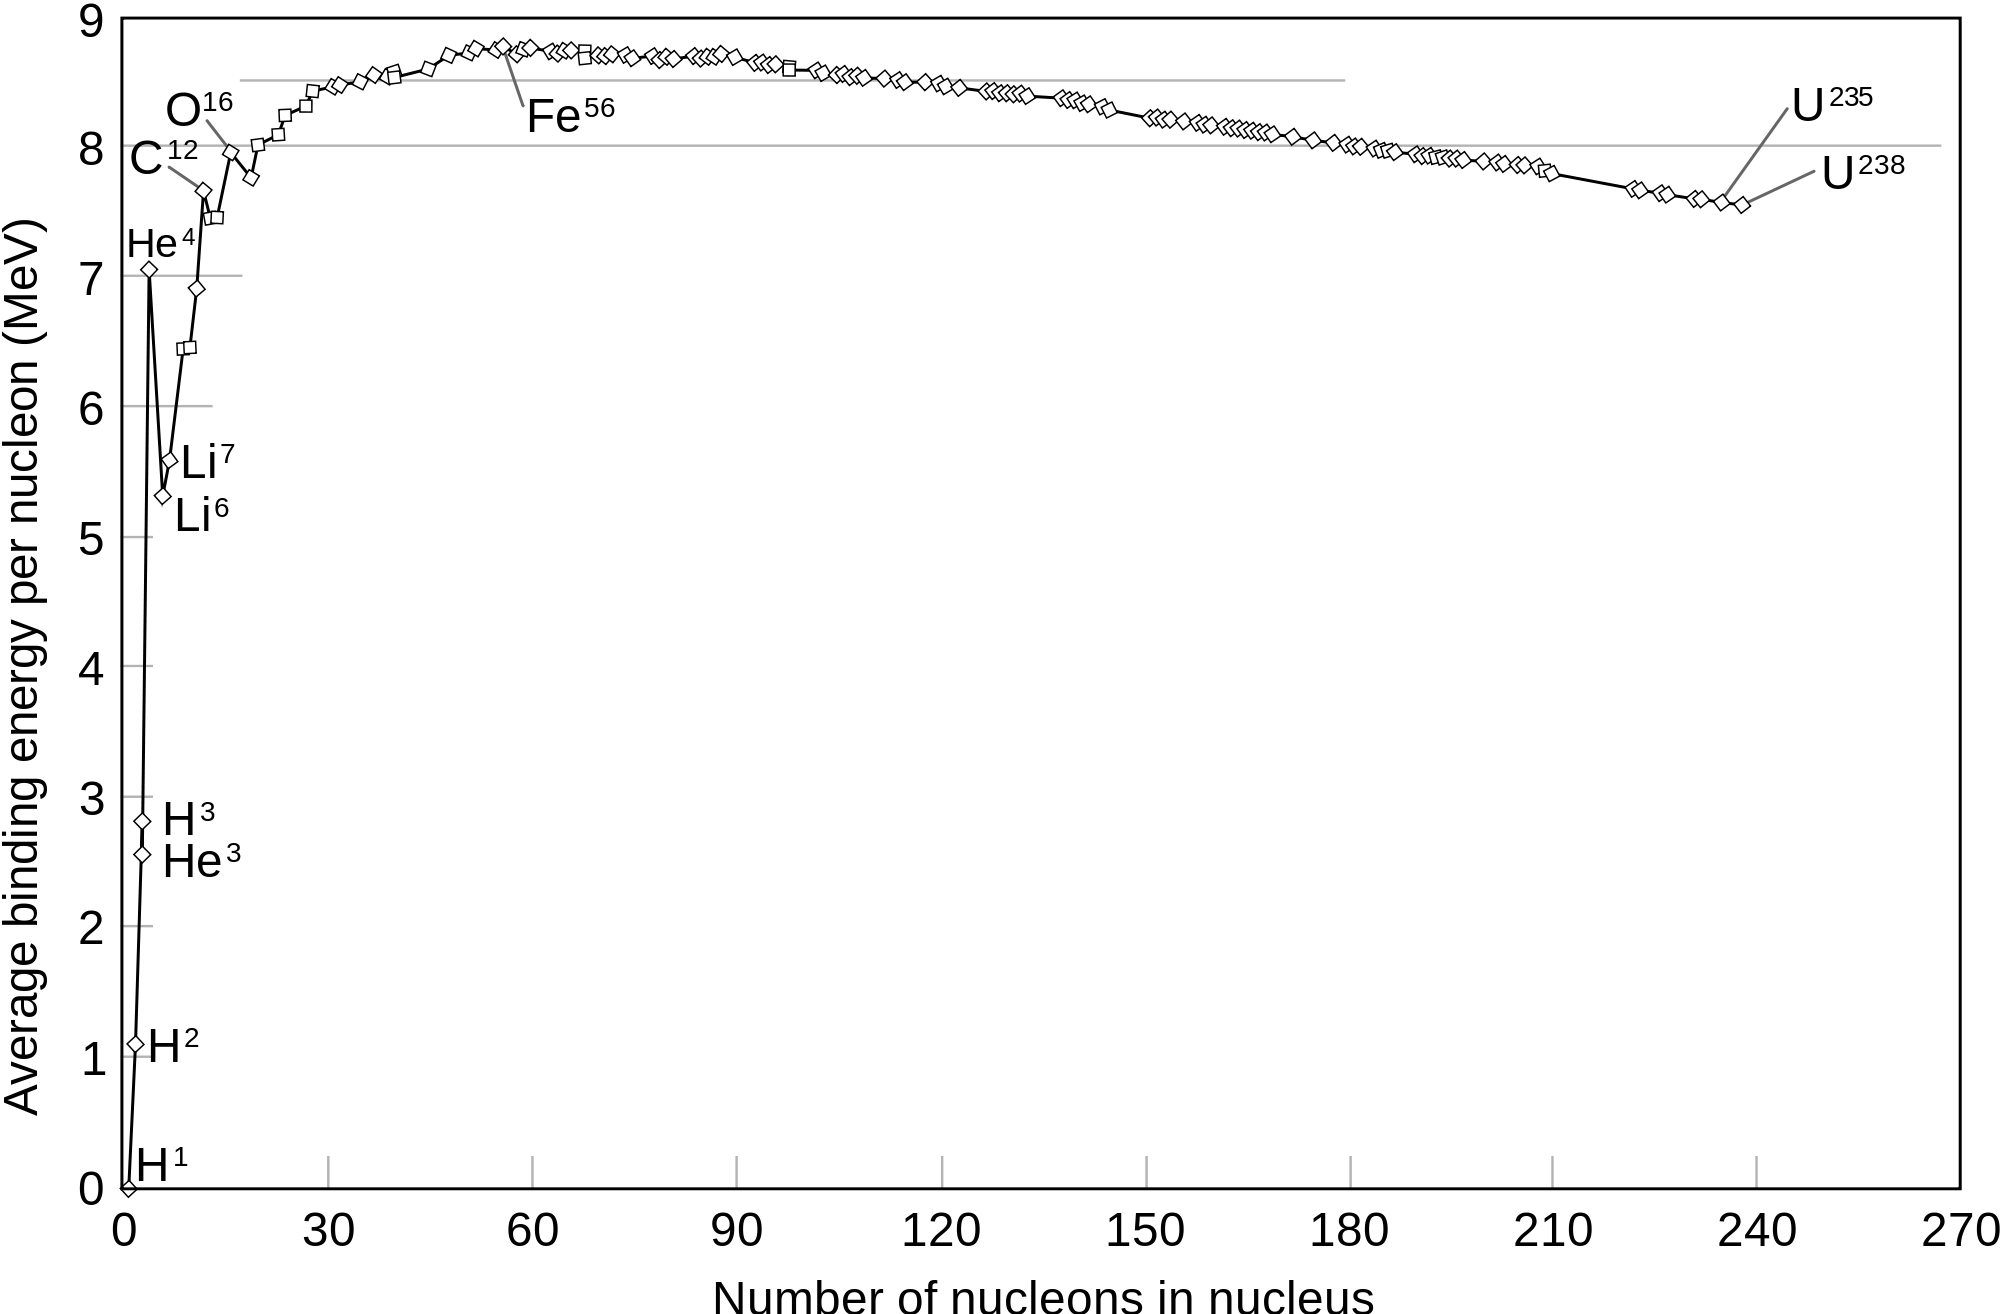
\includegraphics[width=0.6\textwidth]{KernePartikel/binding_energy.png}
  \caption{Bindingsenergi per nukleon som funktion af massetallet, $A$}
  \label{fig:binding}
\end{figure}

Figuren angiver udvalgte kerner, for eksempel He-3 ($Z=2,N=1$), He-4($Z=2,N=2$) og Fe-56 (jern-56, $Z=26,N=30$). Vi kan gøre os følgende observationer; først og fremmest vokser $E_B/A$ stejlt for de lette kerner. Kurven ser ud til at toppe omkring Jern--56. Herefter falder bindingsenergien per nukleon langsomt igen for de tunge kerner. Desuden er kurven heller ikke "glat",  men viser udslag af høje bindingsenergier for bestemte kerner, He--4, Ca--12 (Carbon--12), O--16 (Oxygen--16)... Vi skal senere vende tilbage til, hvorfor netop kernerne  He-4, Ca-12, og O-16 udviser høj bindingsenergi, altså er særlig stabile.

\subsection{Stabile og Ustabile Kerner}
Kerner kan enten være stabile eller ustabile. At en kerne er stabil betyder, at den, ulig de ustabile kerner, ikke er radioaktiv, det vil sige, at den ikke spontant undergår radioaktiv henfald. Når der snakkes om stabile kerner, mener man stabile isotoper, idet det samme element både kan have stabile og ustabile isotoper. Vi kan prøve at plotte de eksperimentelt bestemte stabile isotoper ud fra deres værdier af $Z$ og $N$. Et sådan plot er vist i Figur \ref{fig:stable_iso}.

\begin{figure}[h!]
  \centering
  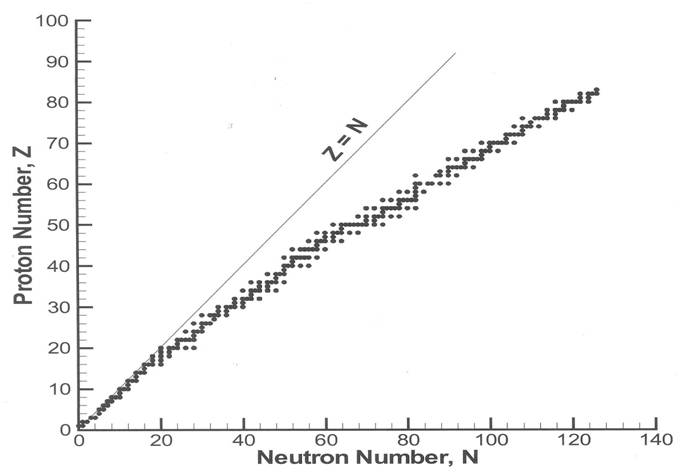
\includegraphics[width=0.6\textwidth]{KernePartikel/stable_nucleides.jpg}
  \caption{Stabile isotoper (markeret som sorte firkanter) og deres værdier af $Z$ og $N$.}
  \label{fig:stable_iso}
\end{figure}

Indtegnet på figuren er også linjen svarende til $Z=N$. Det ses, hvordan de lette kerner (små værdier af $Z$ og $N$) ligger op ad denne linje, men efterhånden som vi bevæger os mod de tungere kerner (højere værdier af $Z$ og $N$), afviges der fra den rette linje, og isotoper med højere $N$ favoriseres over isotoper med højere $Z$. Den snævre region af stabile kerner vist i Figur \ref{fig:stable_iso} kaldes for \emph{stabilitetslinjen} \\
Plottet vist i Figur \ref{fig:known_iso} viser alle kendte isotoper, med de stabile isotoper igen markeret i sort. Det ses, hvordan kerner ikke er fundet til at have vilkårlige antal $Z$ og $N$, eksempelvis ses ingen kerner til at have $Z=50, N=20$ eller $Z=100, N=100$. Generelt er der ingen kerner som udviser meget stor forskel mellem $Z$ og $N$, meget højt protonantal ($Z \gtrsim 80$) eller er ekstremt tunge ($A \gtrsim 200$). 

\begin{figure}[h!]
  \centering
  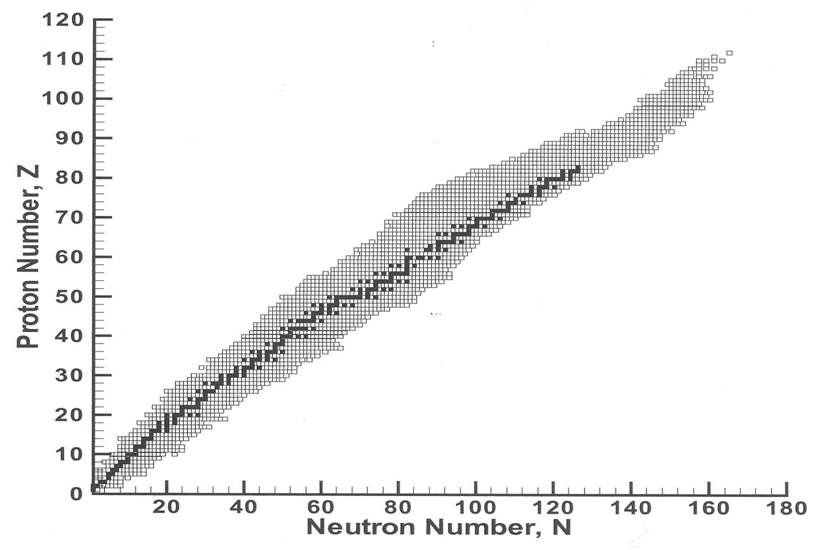
\includegraphics[width=0.6\textwidth]{KernePartikel/known_nucleides.jpg}
  \caption{ Alle kendte isotoper ud fra deres værdier af $Z$ og $N$. Stabile isotoper er markeret som sorte firkanter, mens ustabile isotoper er markeret med lysegrå firkanter}
  \label{fig:known_iso}
\end{figure}


Vi vil komme til at se, at ustabile kerner kan "vinde"  energi ved at undergå radioaktivt henfald og ændre komposition, således at de bevæger sig tættere på stabilitetslinjen i $NZ$-plottet. Eksempelvis vil kerner, som har mange neutroner i forhold til protoner (kernerne, som ligger under stabilitetslinjen) spontant omdanne en af deres neutroner til en proton i det der hedder et $\beta^-$-henfald, mens meget tunge kerner kan brydes op i to mindre kerner, hvoraf én typisk er $^4\text{He}$.  

\subsection{Magiske Tal og Skalmodellen}

Vi skal nu vende de særligt stabile kerner, som viser sig i Figur \ref{fig:binding} ved at have særlig høj $E_B/A$. Denne opførsel kan forudsiges ved at beskrive kernen ud fra et bestemt billede, kaldet skalmodellen, og med denne kan vi forstå, hvorfor eksempelvis $^4\text{He}$ er så stabil.
Skalmodellen minder i princippet om et andet fænomen, I nok har hørt om i forbindelse med elektronskaller. Elektroner bundet i et atom kan ses som at arrangere sig i bestemte "baner" eller skaller om atomkernen. Hver skal kan holde et bestemt antal elektroner, og elektronerne vil generelt fylde skallerne nedefra og op. Atomer, hvis elektronskaller alle er fyldt op, deltager ikke i kemiske reaktioner. Dette kender vi fra ædelgasserne.
Tilbage til skalmodellen og kerne--billedet. Selvom billedet er mere komplekst, så kan kernen på samme måde som atomet siges at bestå af en række skaller og underskaller. Men i stedet for at fylde skallerne op med elektroner, skal skallerne fyldes med protoner og neutroner. Grundet Paulis udelukkelsesprincip, kan der kun eksistere et endeligt antal protoner eller neutroner i en skal. Bestemte antal af $Z$ og $N$ vil på samme måde som elektronerne, svare til fyldte skaller. Ud fra skalmodellen er disse forudset til at være

\begin{equation}
2,8,20,28,50,82,126, ~\text{magiske tal for $Z$ og $N$}.
\label{eq:magicnumbers}
\end{equation}

Disse kaldes for \emph{magiske tal}. Det er altså for disse proton- og neutron-antal, at bindingsenergien per nukleon er usædvanlig høj. Bemærk at selvom $Z=126$ er forudsagt som en "magisk"  kerne, så er denne kerne ikke observeret i naturen. Det er også muligt for en kerne at være dobbelt-magisk, i så fald er både $Z$ og $N$ magiske tal. Dette gælder blandt andet for kernerne

\begin{equation*}
^{4}_{2}\text{He},~~ ^{16}_{~8}\text{O},~~ ^{40}_{20}\text{Ca},~~ ^{48}_{20}\text{Ca},~~  ^{208}_{82}\text{Pb}. 
\end{equation*}

\subsection{Kerners Henfald}

Omkring 90\% af alle kendte kerner er radioaktive og kan derfor henfalde spontant. Som nævnt i det foregående afsnit, vil et henfald af en ustabil kerne bringe kernen tættere på stabilitetslinjen i $NZ$-kortet. For et henfald som ændrer kompositionen af kernen (ændrer $Z$ eller $N$) benævnes den originale kerne som \emph{moder-kernen}, mens slutproduktet kaldes for \emph{datter-kernen}. Et henfald kan foregå spontant (naturligt) såfremt massen af det originale atom (tit kaldet den initiale masse, $M_i$) er større end massen af slutproduktet (den finale masse, $M_f$). I enheder af energi er forskellen mellem de to simpelt skrevet som:

\begin{equation}
Q =(M_i - M_f)c^2.
\label{eq:Qvalue}
\end{equation}

Dette tal kaldes for reaktionens $Q$-værdi. Det ses, at for reaktioner med positiv $Q$-værdi (såkaldt exo-energiske reaktioner) må det gælde at $M_i > M_f$, og det er altså disse reaktioner, som kan foregå. Nedenfor gennemgås nogle almindelige slags henfald; alfa-- og beta--henfald, som ændrer kompositionen af kernerne, og gamma--henfald, som er et indre henfald af et anslået atom, og derfor ikke ændrer $Z$ eller $N$.

\subsubsection{Alfa-henfald}
Et alfa-henfald sker når moderkernen udskiller en alfa-partikel. Skematisk kan vi skrive:
\begin{equation}
\text{alfa--henfald}: ^A_Z\text{X} \rightarrow ^{A-4}_{Z-2}\text{Y} + ^4_2\text{He}.
\label{eq:alfa} 
\end{equation}

Normalt skelner man mellem notationen $\alpha$ (helium--kerne) og $^4_2\text{He}$ (helium--atom). Ved at skrive $^4_2\text{He}$ i reaktionsskemaet angiver man, at der regnes med atomare masser, og ikke kernemasser -- på denne måde er ladningen også bevaret i reaktionen. Anvend derfor den atomare masse af $^4_2\text{He}$ medmindre andet er angivet.

\subsubsection{Beta-henfald}
Der findes tre former for beta-henfald, kaldet beta--minus (skrevet som $\beta^-$), beta-plus ($\beta^+$) og elektronindfangning. Ligesom ved alfa--henfaldet er henfaldet navngivet efter den partikel, der udsendes i reaktionen. En beta--minus--partikel er en elektron. Det er ikke åbenlyst hvordan en kerne kan udsende en elektron, når den kun består af neutroner og protoner, men vi ser, hvordan henfaldet omhandler omdannelsen af en neutron til en proton. Dette slags henfald forekommer derfor for kerner, som har mange neutroner i forhold til protoner (kerner som befinder sig under stabilitetslinjen i $NZ$-plottet vist i Figur \ref{fig:known_iso}). Omdannelsesprocessen forløber således:
\begin{equation}
\text{$\beta^-$-henfald: }n \rightarrow p + e^- + \bar{\nu}_e
\end{equation}
eller skrevet ved brug af kerne-notation:

\begin{equation}
\text{$\beta^-$-henfald: } ^A_Z\text{X} \rightarrow ^A_{Z+1}\text{Y} + e^- + \bar{\nu}_e
\end{equation}

Partiklen angivet som $\bar{\nu}_e$ er en \emph{anti--neutrino} (hvor en neutrino skrives som $\nu_e$ ved det græske bogstav "nu"). Vi skal i kapitlet om partikelfysik gennemgå nogle simple love, der dikterer, hvorfor henfaldet kræver udsendelse af en anti-neutrino, men for nu bliver vi nødt til bare at godtage dens tilstedeværelse. Neutrinoen og anti--neutrinoen er effektivt masseløse, så der skal ikke tages højde for dem under beregning af $Q$--værdi. 

$\beta^+$--henfald forekommer for kerner, som har mange protoner i forhold til neutroner. Her udsendes elektronens anti--partikel, \emph{positronen} ($e^+$), og en neutrino:

\begin{equation}
\text{$\beta^+$--henfald: } p \rightarrow n + e^+ + \nu_e,
\end{equation} 

 som ved brug af kerne--notation skrives som
 
\begin{equation}
\text{$\beta^+$--henfald: } ^A_Z\text{X} \rightarrow ^A_{Z-1}\text{Y} + e^+ + \nu_e.
\end{equation}

Den sidste form for beta--henfald kaldes for elektronindfangning (\emph{eng: electron capture}, forkortet EC). Dette er en proces, hvor kernen "fanger" en af atomets inderste elektroner og omdanner den til en neutron:

\begin{equation}
\text{EC: } p + e^- \rightarrow n + \nu_e,
\end{equation}

som skrives som:

\begin{equation}
\text{EC: } ^A_Z\text{X}~\rightarrow~^A_{Z-1}\text{Y} + \nu_e.
\end{equation}

\subsubsection{Gamma-henfald}
Kerner, som gennemgår et henfald eller en kollision, kan ende i en anslået (exciteret) tilstand. Dette betyder, at kernens nukleoner ikke befinder sig i den lavest mulige energitilstand (kaldet grundtilstanden), men besidder "ekstra" energi i kraft af at befinde sig i en højere energitilstand. For at "falde tilbage"  til grundtilstanden skal kernen give afkald på den ekstra energi, og dette sker under udsendelse af en \emph{foton}, skrevet med symbolet $\gamma$ (det græske bogstav "gamma"). Denne slags henfald kaldes for et gamma-henfald. En foton, også kaldet en lys--kvant, besidder en energi, men ingen ladning. Et gamma-henfald kan derfor ikke ændre på sammensætningen af en kerne, og $A,Z$ og $N$ ændres derfor ikke. En kerne, som er exciteret angives normalt med symbolet " * ". Et gamma--henfald kan derfor skrives skematisk som

\begin{equation}
\text{gamma-henfald: } ^A_Z\text{X}^* \rightarrow ^A_Z\text{X} + \gamma.
\end{equation}
\newpage

\section{Partikelfysik}
\label{cha:partikel}

Partikelfysik er den gren af fysikken, som beskæftiger sig med
universets mindste bestanddele og deres vekselvirkning med hinanden.
Vi har indtil videre stiftet bekendtskab med en del allerede;
elektronen, protonen, neutronen og neutrinoen, og du har måske selv
hørt om partikler som muonen og Higgs--bosonen. Partikelfysikkens
zoologiske have indeholder en bred vifte af partikler, hvoraf de mest
fundamentale partikler er elementarpartiklerne -- partikler, som man
mener ikke kan deles. Heriblandt er elektronen, neutrinoen og
kvarkerne. Kvarker i sammensætning udgør hadronerne, som protonerne og
neutronerne er eksempler på. Dette afsnit vil give et kort overblik
over partiklerne, deres egenskaber og fysikkens indtil videre bedste
bud på et samlet billede af alt i verden, kaldet standardmodellen.

\subsection{Standardmodellen}
Standardmodellen er teorien om de elementare partikler og hvordan de
fire fundamentale naturkræfter -- tyngdekraften, den elektromagnetiske
kraft og den stærke og svage kernekraft -- vekselvirker.

\subsubsection{Partikler og anti-partikler}
Der arbejdes her med tre egenskaber for partiklerne: masse, ladning og
\emph{spin}. Spin er en kvantemekanisk egenskab for en partikel, som
ikke har nogen analog i den makroskopiske fysiske verden\footnotemark,
men det besidder altid en bestemt størrelse og en retning, og er
vigtigt, hvis man vil regne kvantemekanisk på partiklerne.
\footnotetext{Nogle bøger i gymnasiet beskriver en partikels spin, som
  at man kan forestille sig, at partiklen drejer om sig selv på samme
  måde som at Jorden roterer, men dette billede er fundamentalt
  forkert og skal slettes fra din bevidsthed så hurtigt som muligt.}
Alle partikler har en \emph{antipartikel}. En antipartikel er ens i
alle henseender med sin partikel bortset fra sin ladning (og andre
tekniske egenskaber, som vi ikke vil komme ind på her). Den negativt
ladede elektron, $e^-$, har antipartiklen kaldet positronen (også
nogle gange kaldet anti-elektronen), $e^+$. De to partikler har samme
masse og spin, men modsatte ladninger. Hvis en elektronen og en
positron ''møder'' hinanden, ophæver de hinanden og de eksisterer ikke
længere. Dette kaldes for en \emph{annihilation}. På grund af energi--
og impulsbevarelse, bliver der i en annihilation altid skabt partikler
til at bære den overskydende energi væk. En annihilation mellem en fri
elektron og en positron skaber to fotoner:
\begin{equation}
e^- + e^+ \rightarrow \gamma + \gamma 
\end{equation}
Fotonerne har ingen masse, men får sin energi fra masserne af
elektronen og positronen gennem Einsteins formel $E=mc^2$, der giver
en ækvivalens mellem energi $E$ og masse $m$, idet $c$ blot er en
naturkonstant (lysets fart i vakuum). For visse partikler gælder det,
at de er sin egen antipartikel, fx fotonen. To fotoner kan eksempelvis
annihilere i den omvendte reaktion:
\begin{equation}
\gamma + \gamma \rightarrow e^- + e^+,
\end{equation}
så længe reaktionen overholder energi-- og impulsbevarelse.

Standardmodellens elementare partikler er vist skematisk i Figur
\ref{fig:standard}. De er leptonerne, kvarkerne (eng: \emph{quarks}),
de vekselvirkende eller kraftbærende partikler (kaldet
\emph{gauge-bosoner}) og Higgs-bosonen.
\begin{figure}[h!]
  \centering
  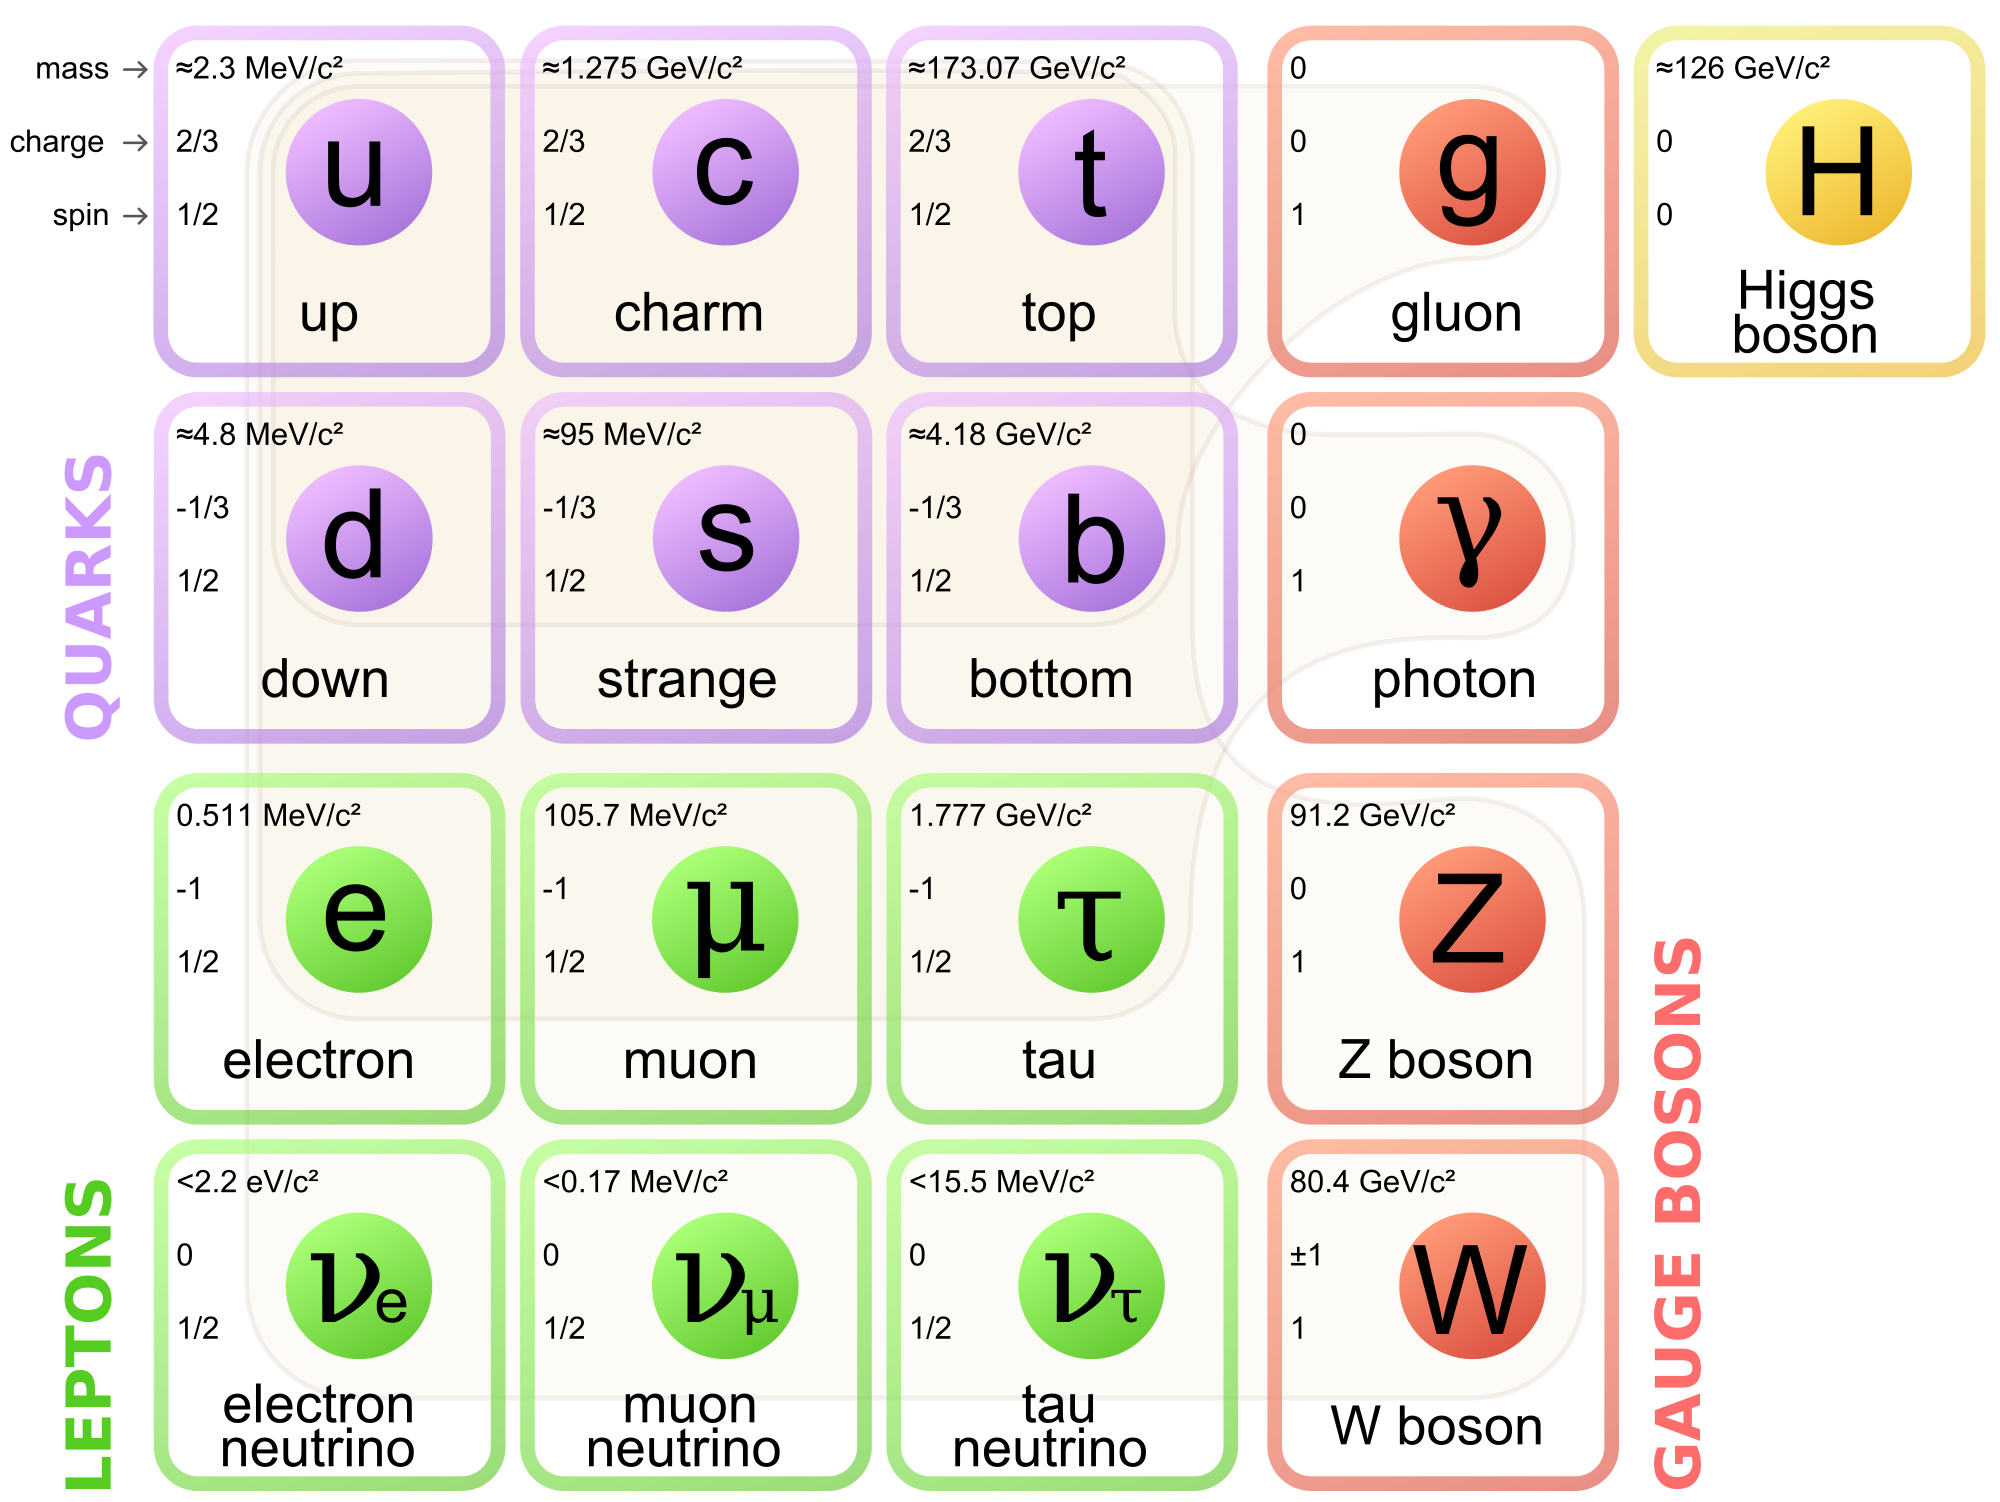
\includegraphics[width=0.6\textwidth]{KernePartikel/fig_p/standard.png}
  \caption{ Standardmodellens elementarpartikler: leptonerne,
      kvarkerne, gauge-bosonerne og Higgs-bosonen. Til venstre i hver
      kasse ses partiklens masse, ladning og spin.}
  \label{fig:standard}
\end{figure}

\subsubsection{Leptoner}
Leptonerne er en gruppe af elementare partikler, som ikke vekselvirker
gennem den stærke kernekraft. Alle leptoner har spin $s = 1/2$, og er
derfor det, der kaldes \emph{fermioner}.

Leptonerne er overordnet delt ind i tre grupper, kaldet
generationer. Én generation af leptoner består af en ladet partikel og
en neutral partikel. Vi har allerede stiftet bekendtskab med én
generation af leptoner, nemlig den ladede elektron, $e^-$ og den
neutrale (elektron)neutrino, $\nu_e$. Næste generation af leptoner
udgøres af \emph{muonen} (skrevet som det græske bogstav 'mu', $\mu$)
og muon--neutrionen, $\nu_\mu$. Sidste generation af leptoner er den
tunge partikel \emph{tau} (skrevet som det græske bogstav, 'tau',
$\tau$) og tau--neutrinoen, $\nu_\tau$ . Muonen og tau--partiklen, der er
meget massive i forhold til elektronen, er ustabile og vil derfor
hurtigt henfalde til elektroner. De kan på grund af deres høje masser
kun dannes i høj--energi kollisioner, som dem der foregår i
partikelacceleratorer eller reaktioner involverende kosmisk stråling
(husk, at masser og energi er det samme i partikelfysikken, så det
kræver meget energi at skabe tunge partikler).

Leptonerne, inklusiv antipartiklerne $e^+,\bar{\mu}, \bar{\tau},
\bar{\nu}_e...$ kan påvirkes af tyngdekraften, den elektromagnetiske
kraft og den svage vekselvirkning.

\subsubsection{Kvarkerne}
Kvarkerne er de partikler som kan sammensættes til blandt andet
protonerne og neutronerne. En speciel egenskab for kvarkerne gør, at
de aldrig kan findes isoleret, og kvarkerne kan derfor aldrig
observeres direkte. De er spin 1/2-partikler ligesom leptonerne, og
besidder forskellige brøkdele af elementarladningen, som det ses af
Figur \ref{fig:standard}.

De er navngivet up, down, charm, strange, top og bottom med symbolerne
u, d, c, s, t og b. En vilkårlig kvark angives som q, og en antikvark
som $\bar{\text{q}}$. Kvarkernes egenskaber og evidens for deres
eksistens er opdaget ved at studere hadroner (altså de partikler, som
kvarkerne er byggesten for, se afsnit \ref{sec:hadron}), og de første
kvarker blev studeret i slutningen af 1960'erne, mens den sidste og
tungeste kvark, top--kvarken, blev opdaget i 1995.

Kvarkerne er de eneste partikler som kan vekselvirke gennem alle fire
fundamentale kræfter.

\subsection{De Fundamentale Kræfter og Gauge--bosoner}
Standardmodellen arbejder med fire fundamentale kræfter. Tabel
\ref{tab:forces} viser de fire former for vekselvirkning, og deres
styrke relativ til den stærkeste kraft, den stærke vekselvirkning.

\begin{table}[h]
\centering
    \begin{tabular}{l|l|l|l}
    Vekselvirking    & Relativ styrke  & Rækkevidde                   & Partikel                   \\ \hline
    Stærk            & 1               & kort ($\sim \SI{1}{fm}$)     & gluon, g                   \\
    Elektromagnetisk & $\frac{1}{137}$ & lang ($1/r^2$)               & foton, $\gamma$            \\
    Svag             & $\sim 10^{-9}$  & kort  ($\sim \SI{0.001}{fm}$) & $\text{W}^\pm, \text{Z}^0$ \\
    Gravitationel    & $\sim 10^{-38}$ & lang ($1/r^2$)               & graviton                   \\
    \end{tabular}
    \caption{De fire fundamentale kræfter og deres
        vekselvirkningspartikler, hvoraf gravitonen endnu ikke er
        eksperimentelt bekræftet.}
    \label{tab:forces}
\end{table}

Den elektromagnetiske vekselvirkning og tyngdekraften kendes fra
klassisk fysik, som kræfter, hvis styrke afhænger af afstanden mellem
de vekselvirkende objekter som $1/r^2$. Den stærke vekselvirkning, er
ansvarlig for den stærke kernekraft, som holder nukleonerne i kernen
sammen. Den har en kort rækkevidde, typisk omkring udstrækningen af en
kerne. I følgende afsnit skal vi lære, at kvarkerne vekselvirker med
hinanden ved hjælp af den stærke vekselvirking. Den svage
vekselvirkning er ansvarlig for beta--henfald, og henfaldet af ustabile
partikler såsom leptonerne.

Standardmodellen beskriver vekselvirkninger gennem de fundamentale
kræfter som udvekslingen af en partikel kaldet en
gauge-boson. Forestil dig to elektroner, som er på vej til at
mødes. De vil frastøde hinanden på grund af deres ladning, men hvordan
ved elektronerne at den anden elektron er til stede? Det ved de fordi
der sker en udveksling af en gauge-boson, i dette tilfælde fotonen.

I dette billede ''bærer'' eksempelvis fotonen den elektromagnetiske
vekselvirkning. Det betyder, at to partikler som interagerer
elektromagnetisk, vil udveksle en foton. De andre gauge-bosoner er
\emph{gluonen}, g, som bærer den stærke vekselvirning og W-- og
Z--partiklerne, som udveksles i reaktioner involverende den svage
kernekraft. Modsat gluonen og fotonen, har Z-- og W--bosonerne masse
(man siger, at de er massive). Z--bosonen er uden ladning, mens
W--bosonen enten kan have positiv eller negativ ladning skrevet
henholdsvis som $\text{W}^+$ og $\text{W}^-$.

Når en gauge--boson udveksles mellem to partikler -- altså når to
partikler vekselvirker gennem en fundamental kraft -- siger man, at
partiklen er \emph{virtuel}. At en partikel er virtuel betyder, at den
''matematisk'' er til stede, men ikke fysisk kan observeres.  Gauge-bosoner har altid et heltalligt
spin, $s = 0,1,2,\dots$

Standardmodellen er en uhyre god fysisk teori, og har gang på gang
vist sig at give korrekte forudsigelser om forskellige
eksperimenter. Desværre har den ét stort problem: Teorien indeholder
ikke tyngdekraften, så standardmodellen indeholder faktisk kun tre ud
af de fire fundamentale naturkræfter. Man kan fikse problemet ved at
tilføje en hypotetisk graviton--partikel, der skulle bære den
gravitationelle vekselvirkning. En komplet fysisk teori må
naturligvis indeholde alle fire naturkræfter, og indtil videre er der
ingen troværdig fysisk teori, der formår dette. Der findes dog
eksotiske bud på sådanne komplette teorier, såsom strengteori og
supersymmetri, men disse har andre store problemer, så der kun er få
fysikere, der tror på dem.

\subsubsection{Higgs--bosonen}
Higgs--bosonen er en partikel, hvis eksistens var forudsagt inden den
blev opdaget i 2013. Higgs--partiklen skaber et felt kaldes
Higgs-feltet, fra hvilket massive partikler får deres masse
fra. Higgs--feltet var en af mange teorier omkring, hvordan masse
skabes, og kan forklare, hvorfor Z og $\text{W}^\pm$ har masse,
hvilket ellers ikke umiddelbart var forventet for
gauge--bosoner. Higgs--partiklen er meget tung, og kræver derfor stor
energi for at kunne skabes i partikelacceleratorer. Derfor er det også
først for nyligt, at man kunne producere partiklen. Efter sin dannelse
vil den meget hurtigt henfalde til lettere partikler.

\subsection{Kvarker i Sammensætning -- Hadroner}
\label{sec:hadron}
Vi lærte i forrige afsnit, at kvarker ikke kan eksistere i
isolation. Kvarker bindes i stedet sammen via den stærke kernekraft i
systemer og danner sammensatte partikler. De sammensatte partikler
(eng: \emph{composite particles}) kaldes samlet set for
\emph{hadroner}.  Der eksisterer to typer hadroner: baryonerne og
mesonerne. Baryonerne er sammensatte partikler bestående af tre
kvarker, mens mesonerne består af et kvark--antikvark--par. Dette er
illustreret i Figur \ref{fig:baryonmeson}.
\begin{figure}[htb]
  \centering
  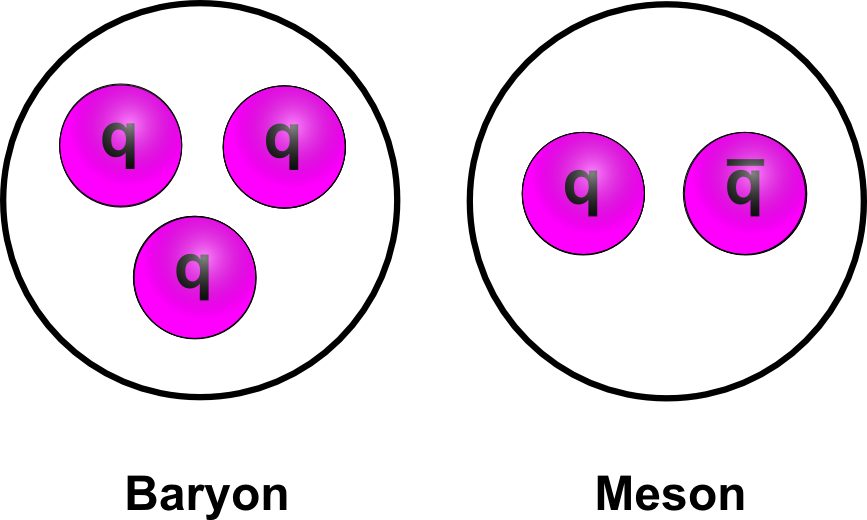
\includegraphics[width=0.3\textwidth]{KernePartikel/fig_p/baryonmeson.png}
  \caption{ Baryoner består af tre kvarker, mens mesoner
      består af en kvark og en antikvark, f.eks. pionen, $\pi^+$, hvis
      kvarkindhold er én u-kvark og én anti-d-kvark, eller
      b-eta-mesonen, $\eta_b$, hvis kvark indhold er én b-kvark og én
      anti-b-kvark.}
    \label{fig:baryonmeson}
\end{figure}
Protoner og neutroner er eksempler på baryoner. Deres sammensætning er
vist i Figur \ref{fig:protonneutron}.
\begin{figure}[htb]
  \centering
  \includegraphics[width=0.3\textwidth]{KernePartikel/fig_p/composite.png}
  \caption{ Protonen og neutronen består af hver tre
      kvarker. Deres antipartikler består af antikvarkerne.}
  \label{fig:protonneutron}
\end{figure}
En proton består af to u--kvarker og én d--kvark, mens neutronen består
af to d--kvarker og én u--kvark. Vi kan forstå mange af deres egenskaber
ved at se på deres kvarksammensætning. Den samlede ladning af
kvarkerne i protonen kombineres til $1$ elementarladning, mens
kvarkerne i neutronen kombineres til ladning 0. Da forskere fandt ud
af, at neutronen besad en magnetisk egenskab kaldet et \emph{magnetisk
  moment}, var det en gåde for dem, hvordan det kunne lade sig gøre
for en neutral partikel, men nu ser vi, hvordan dette skyldes de
magnetiske egenskaber for neutronens individuelle kvarker, som jo
netop har ladning. Vi ser også, hvordan masserne af protonen og
neutronen (omkring \SI{930}{MeV/c^2}) er meget større end massen af de
individuelle up- og down-kvarker, der hver kun vejer \SI{2,3}{MeV/c^2}
og \SI{4,8}{MeV/c^2}), hvor den manglende masse kommer fra
gluonfeltet, som binder kvarkerne sammen. Baryonernes og mesonernes
antipartikler består simpelt af antikvarkerne i stedet for for kvarker
(vist i Figur \ref{fig:protonneutron}).

\subsection{Partikelreaktioner}
Under udarbejdelsen af standardmodellen, så man, hvordan visse
vekselvirkninger og henfald skete ofte, mens andre fandt sted med
langt mindre sandsynlighed eller slet ikke -- såkaldte \emph{forbudte}
reaktioner. Studiet af de forekommende reaktioner har ledt til en
række bevarelseslove, som dikterer hvilke reaktioner, som kan
forekomme, og hvilke der ikke kan. Der skal vanskeligt matematik til
for at regne på reaktionerne, men de kan simpelt visualiseres ved
brugen af såkaldte Feynman-diagrammer.
 
\subsection{Bevarelseslove}
I fysikken dikterer en bevarelseslov at en størrelse ikke ændrer sig
over tid. De fleste har allerede stiftet bekendtskab med koncepter som
energi--, impuls-- og ladningsbevarelse, som også dikterer interaktioner
mellem partikler. Ud over disse bevarelseslove er to andre størrelser
i partikelfysikken bevarede, nemlig \emph{baryon--tal} og
\emph{lepton--tal}. Disse tal kan ses lidt ligesom bevarelsen af den
samlede ladning i en reaktion. Idéen er, at alle baryoner besidder
baryontallet $B=1$, mens deres antipartikler besidder
$B=-1$. Alternativt kan man sige at kvarker har $B=1/3$, mens
antikvarker har $B=-1/3$. Alle partikler som ikke er dannet af kvarker
har automatisk $B=0$. Et eksempel kan være reaktionen:
\begin{equation*}
p + n \not\rightarrow p + \mu^+ + \mu^- .
\end{equation*}
Ladningen er bevaret i denne reaktion, men baryon--tallet er ikke
bevaret, idet vi på højresiden har $B=1+1$, mens vi på venstresiden
har $B=1$, da muonerne begge har $B=0$. Reaktionen vil altså ikke
forekomme!

Lepton-tallet fungerer på samme måde. Her har alle medlemmmer af
lepton--familien ($e^-,\nu_e, \mu^-$, \dots) lepton--tal $L=1$, mens
deres antipartikler ($e^+, \bar{\nu}_e, \mu^+$, \dots) har $L=-1$. Man
skelner også mellem lepton--tal for de forskellige generationer,
skrevet $L_e, L_\mu,L_\tau$ for henholdsvis elektronen, muonen og
tau--partiklen og deres neutrinoer. Disse skal også være bevaret
individuelt.\footnote{Dette er faktisk en sandhed med modifikationer,
  fordi bevarelsen af de enkelte generationers leptontal kan brydes i
  visse tilfælde, men det er meget usandsynligt, så vi vil antage, at
  de altid er bevarede.} Et eksempel er henfaldet af en neutron:
\begin{equation*}
n \rightarrow \bar{p} + e^- + \bar{\nu_e}.
\end{equation*} 
Neutrinoer interagerer så lidt med stof, at de er meget svære at
detektere. Derfor kunne man, baseret på observationer, fristes til at
tro, at reaktionen forløb som $n \rightarrow \bar{p} + e^-$, men dette
passer ikke med den energi, som anti--protonen og elektronen besidder
efter et sådant henfald. Der må være en tredje partikel til
stede. Anti--neutrinoens tilstedeværelse bevarer både energi og
lepton--tal i henfaldet af en neutron.

\subsection{Feynman--Diagrammer}
\label{sec:feyman}
Feynman--diagrammer, udviklet af den berømte amerikanske fysiker
Richard Feynman (1918-1988), er visuelle repræsentationer af
vekselvirkningen mellem partikler. Deres enkelhed gør dem til et
must-have i alle partikelfysikeres værktøjskasse, og de kan anvendes
og forstås uden kompliceret matematik. Dette afsnit gennemgår først
fremgangsmåden for at konstruere et feynman-diagram, og dernæst den
underlæggende fysiske betydning. Reglerne er meget simple!

\subsubsection{Basis konstruktion af feynman-diagrammer}

\begin{enumerate}

\item Først og fremmest arbejdes der med to slags symboler: den lige
  linje med en pil og den bugtede linje:
	\begin{minipage}[c]{\textwidth}
	\centering
     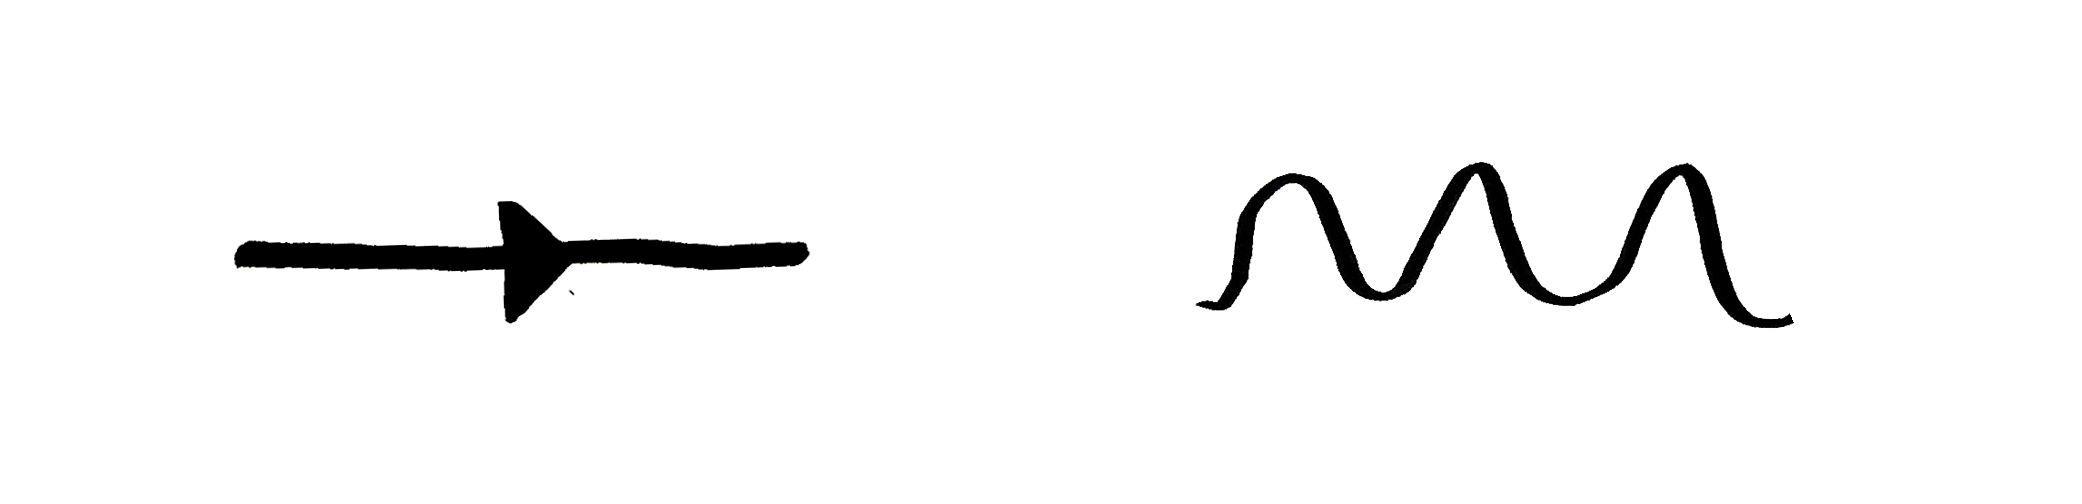
\includegraphics[width=6 cm]{KernePartikel/fig_p/symbols.png}
	\end{minipage}
Pilen kan både pege den ene og den anden vej!

\item De to slags linjer kan forbindes, men kun hvis to linjer med
  pile forbindes med en enkelt bugtet linje. Således:
	\begin{minipage}[c]{\textwidth}
	\centering
     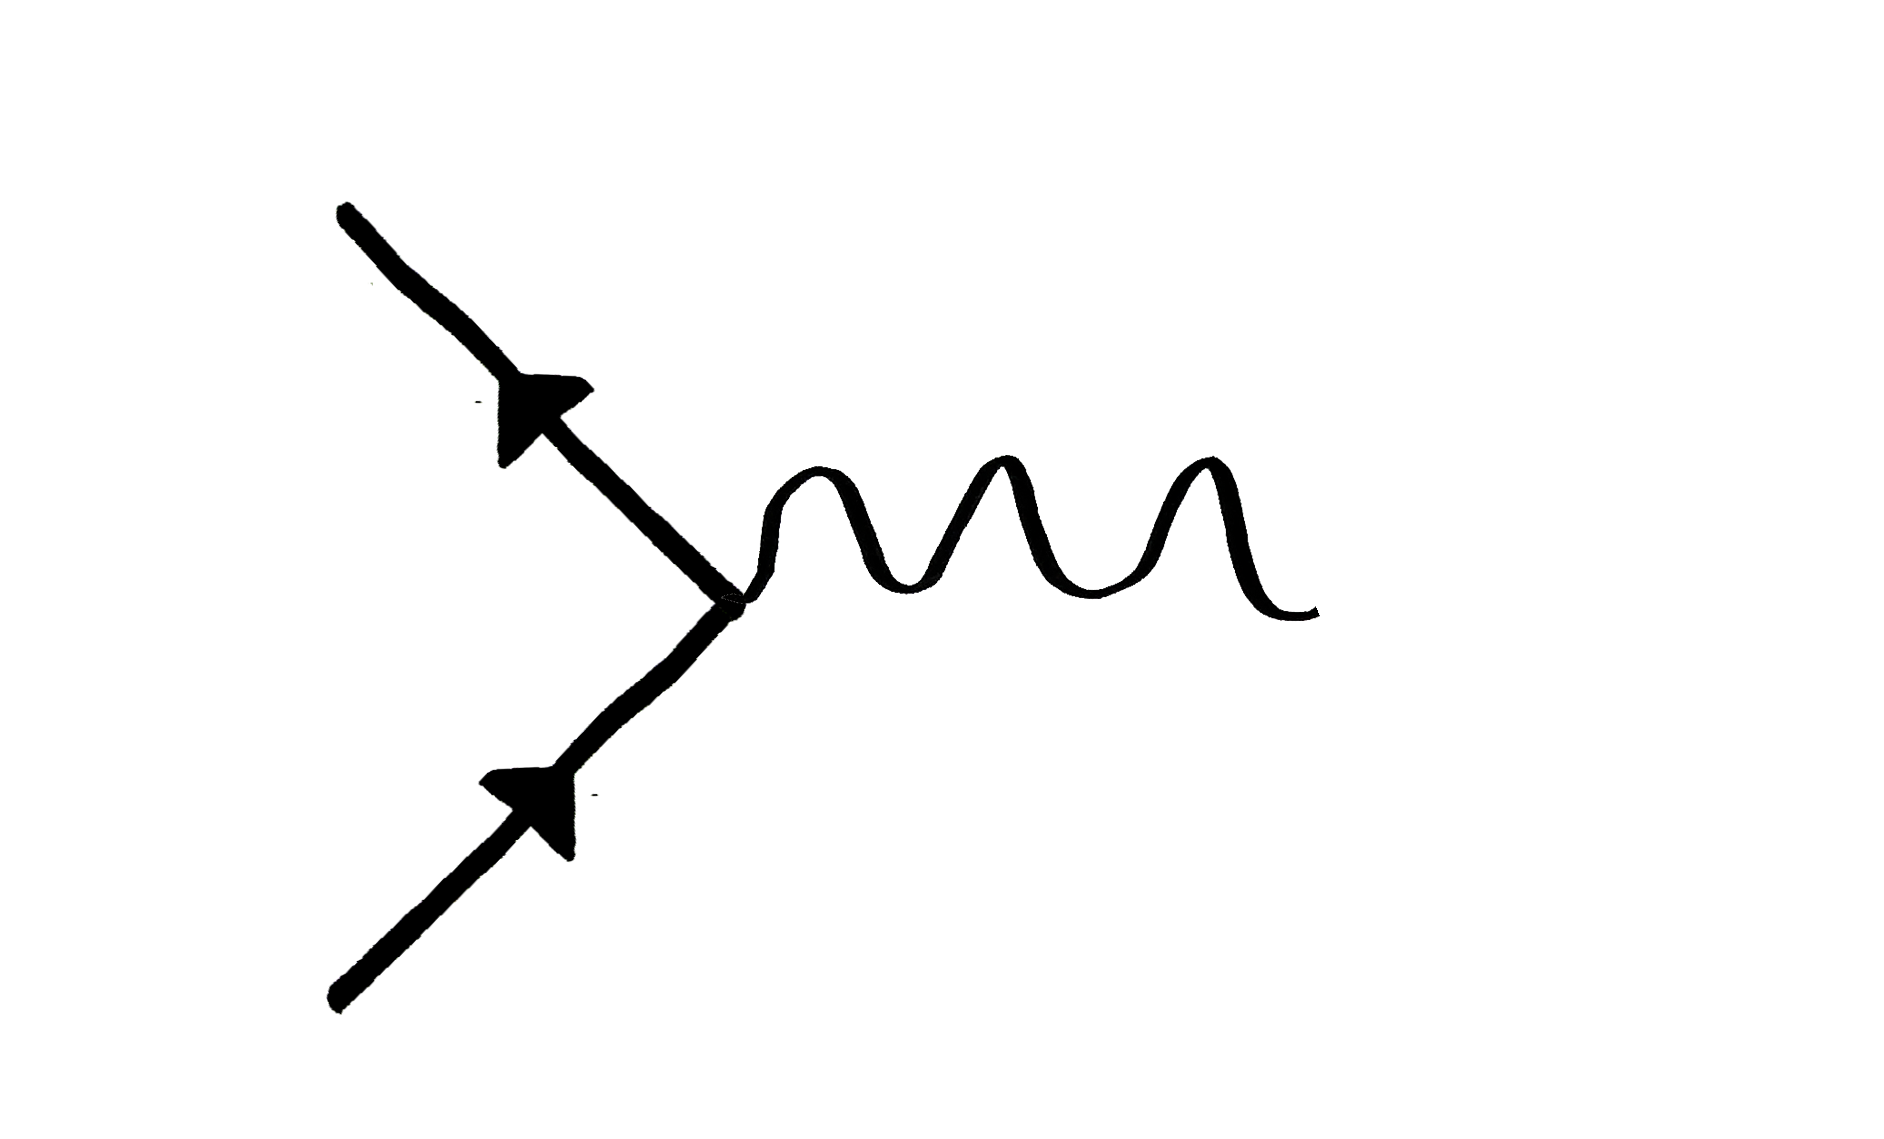
\includegraphics[width=5 cm]{KernePartikel/fig_p/QEDvertex2.png}
	\end{minipage}
        Det punkt, som kombinerer de tre linjer kaldes for et
        \emph{vertex}. Læg mærke til retningen for pilene! Det skal
        gøres således, at \emph{ hver gang en pil peger mod et vertex,
          skal der være en pil, som peger væk fra vertexet}.
\end{enumerate}
Hvad betyder det, fysisk set?  Hver linje i regel (1) er en
partikel. Linjerne med pile er fermioner (elektroner, kvarker, osv.),
mens den bugtede linje kan repræsentere en boson (fotonen, gluonen,
osv.). Dog anvender man normalt forskellige symboler for de
forskellige slags vekselvirkninger, mere om det i opgaveafsnittet.
Vertexet (knudepunktet) er en vekselvirkning/interaktion. Virtuelle partikler eksisterer mellem to vertexer. 

Diagrammerne fortæller en historie om partiklernes vekselvirkning. Vi læser dem fra
venstre mod højre,som det er illustreret i Figur \ref{fig:axis}.
\begin{figure}[h!]
  \centering
  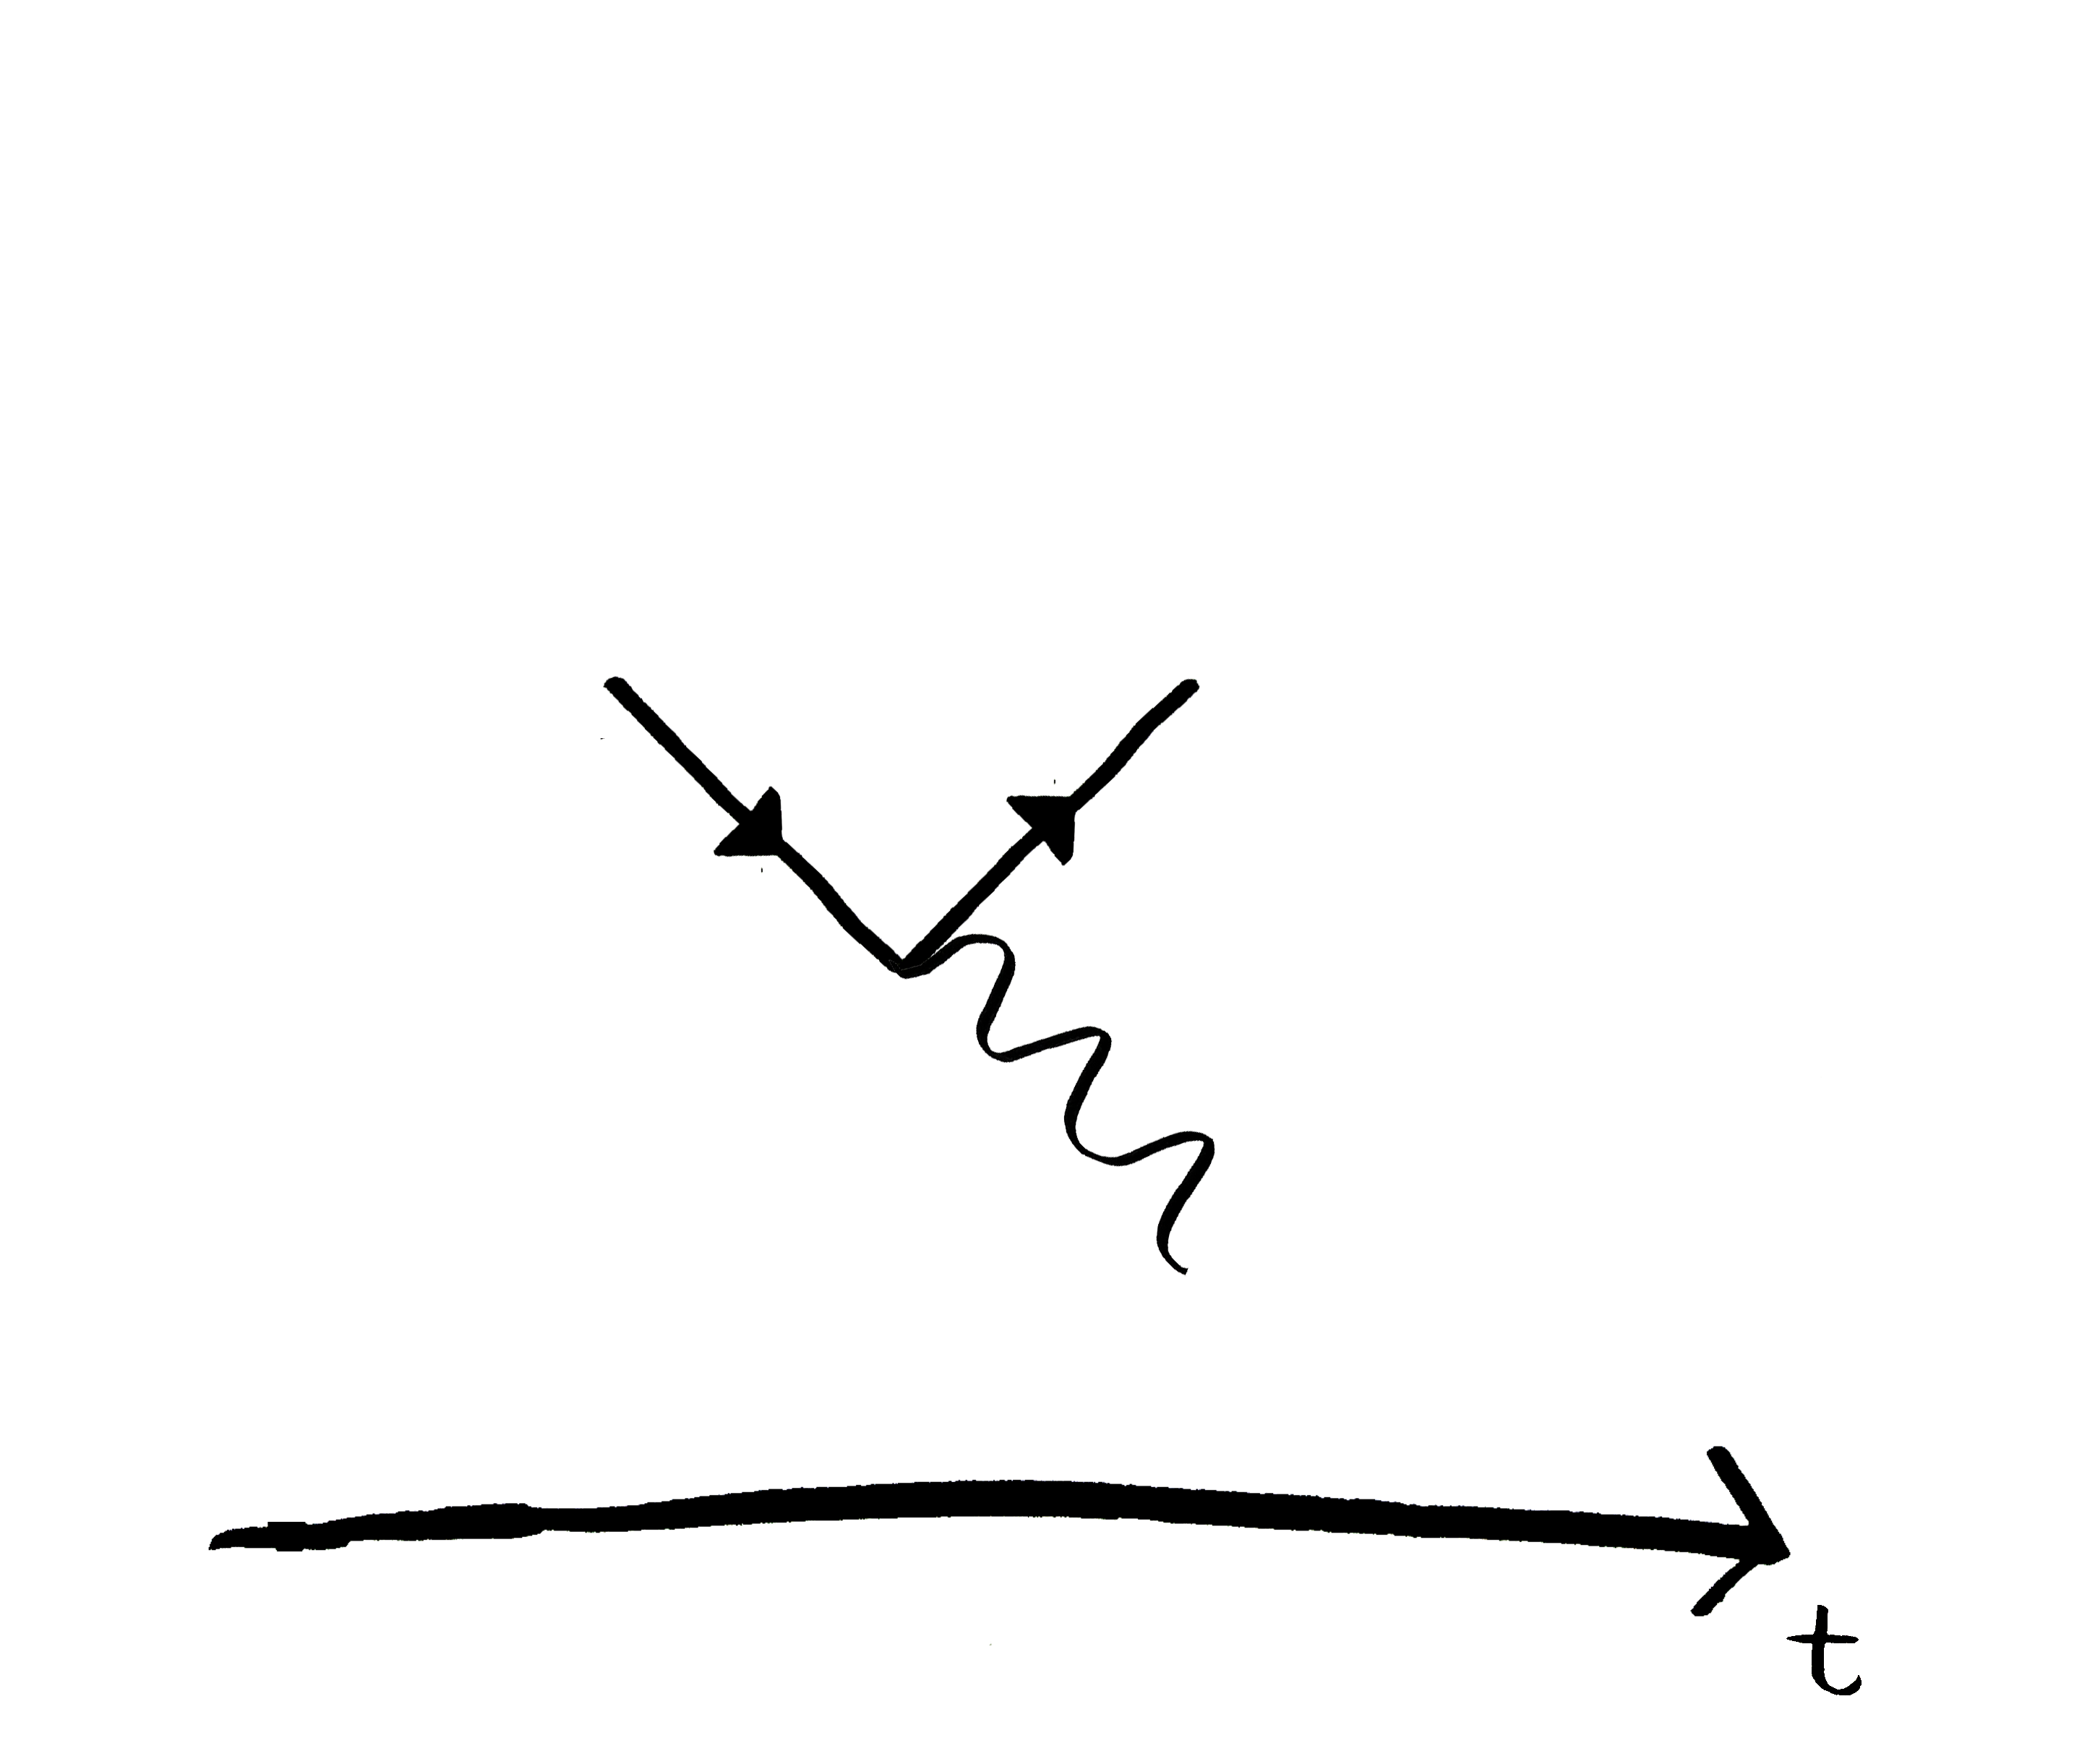
\includegraphics[width=0.3\textwidth]{KernePartikel/fig_p/axis2.png}
  \caption{ Feynman-diagrammer har tiden ad $x$-aksen.}
  \label{fig:axis}
\end{figure}
Normalt tegner man ikke aksen på, som det er gjort i Figur
\ref{fig:axis}, men det kan for nogle være en hjælp, så gør hvad du
føler dig tryg ved. At det er vigtigt at være opmærksom på, at
feynman--diagrammer læses fra venstre mod højre kan illustreres i et
eksempel. Vi kigger her på vekselvirkningen involverende tre
partikler: en elektron, positron og en foton.
\begin{figure}[h!]
  \centering
  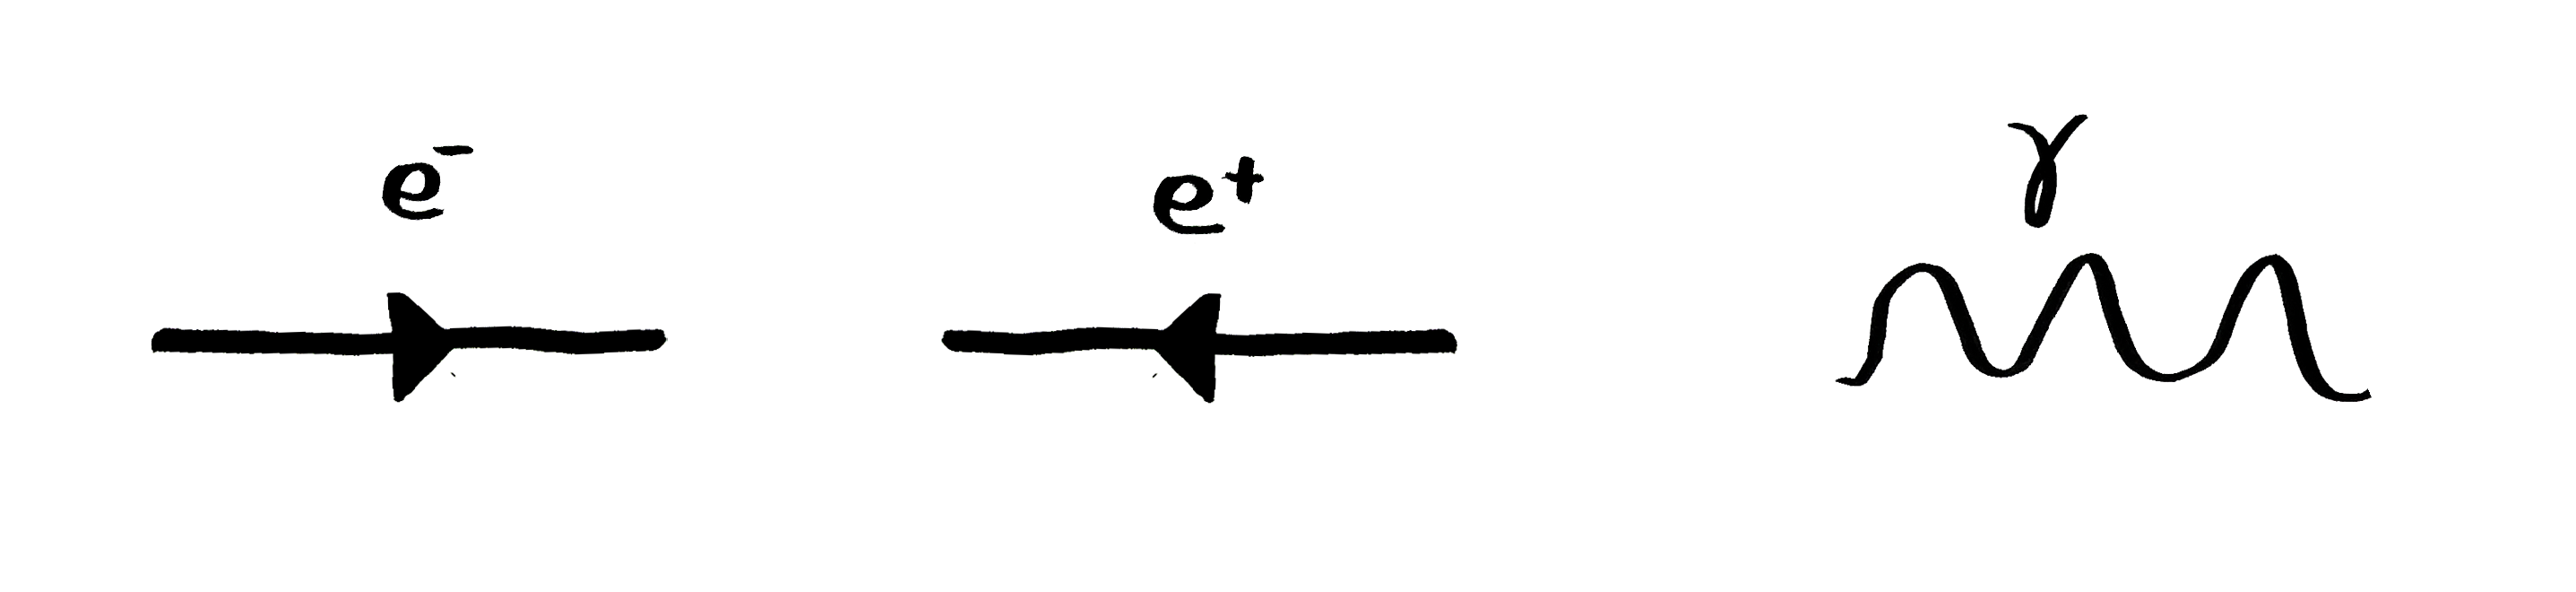
\includegraphics[width=8 cm]{KernePartikel/fig_p/elektron_positron2.png}
  \caption{Elektronen, positronen og en foton illustreret.}
  \label{fig:elektron_positron}
\end{figure}
Læg mærke til, at vi skelner mellem elektronen og dens antipartikel
ved retningen på pilene: \emph{partikler har pile i retning med
  tidsudviklingen og antipartikler har pile modsat
  tidsudviklingen}. Dette betyder \emph{ikke} at anti--partikler bevæger sig
bagud i tid, det er kun et spørgsmål om, hvordan man kan skelne mellem
dem og partiklerne.
\begin{figure}[h!]
  \centering
  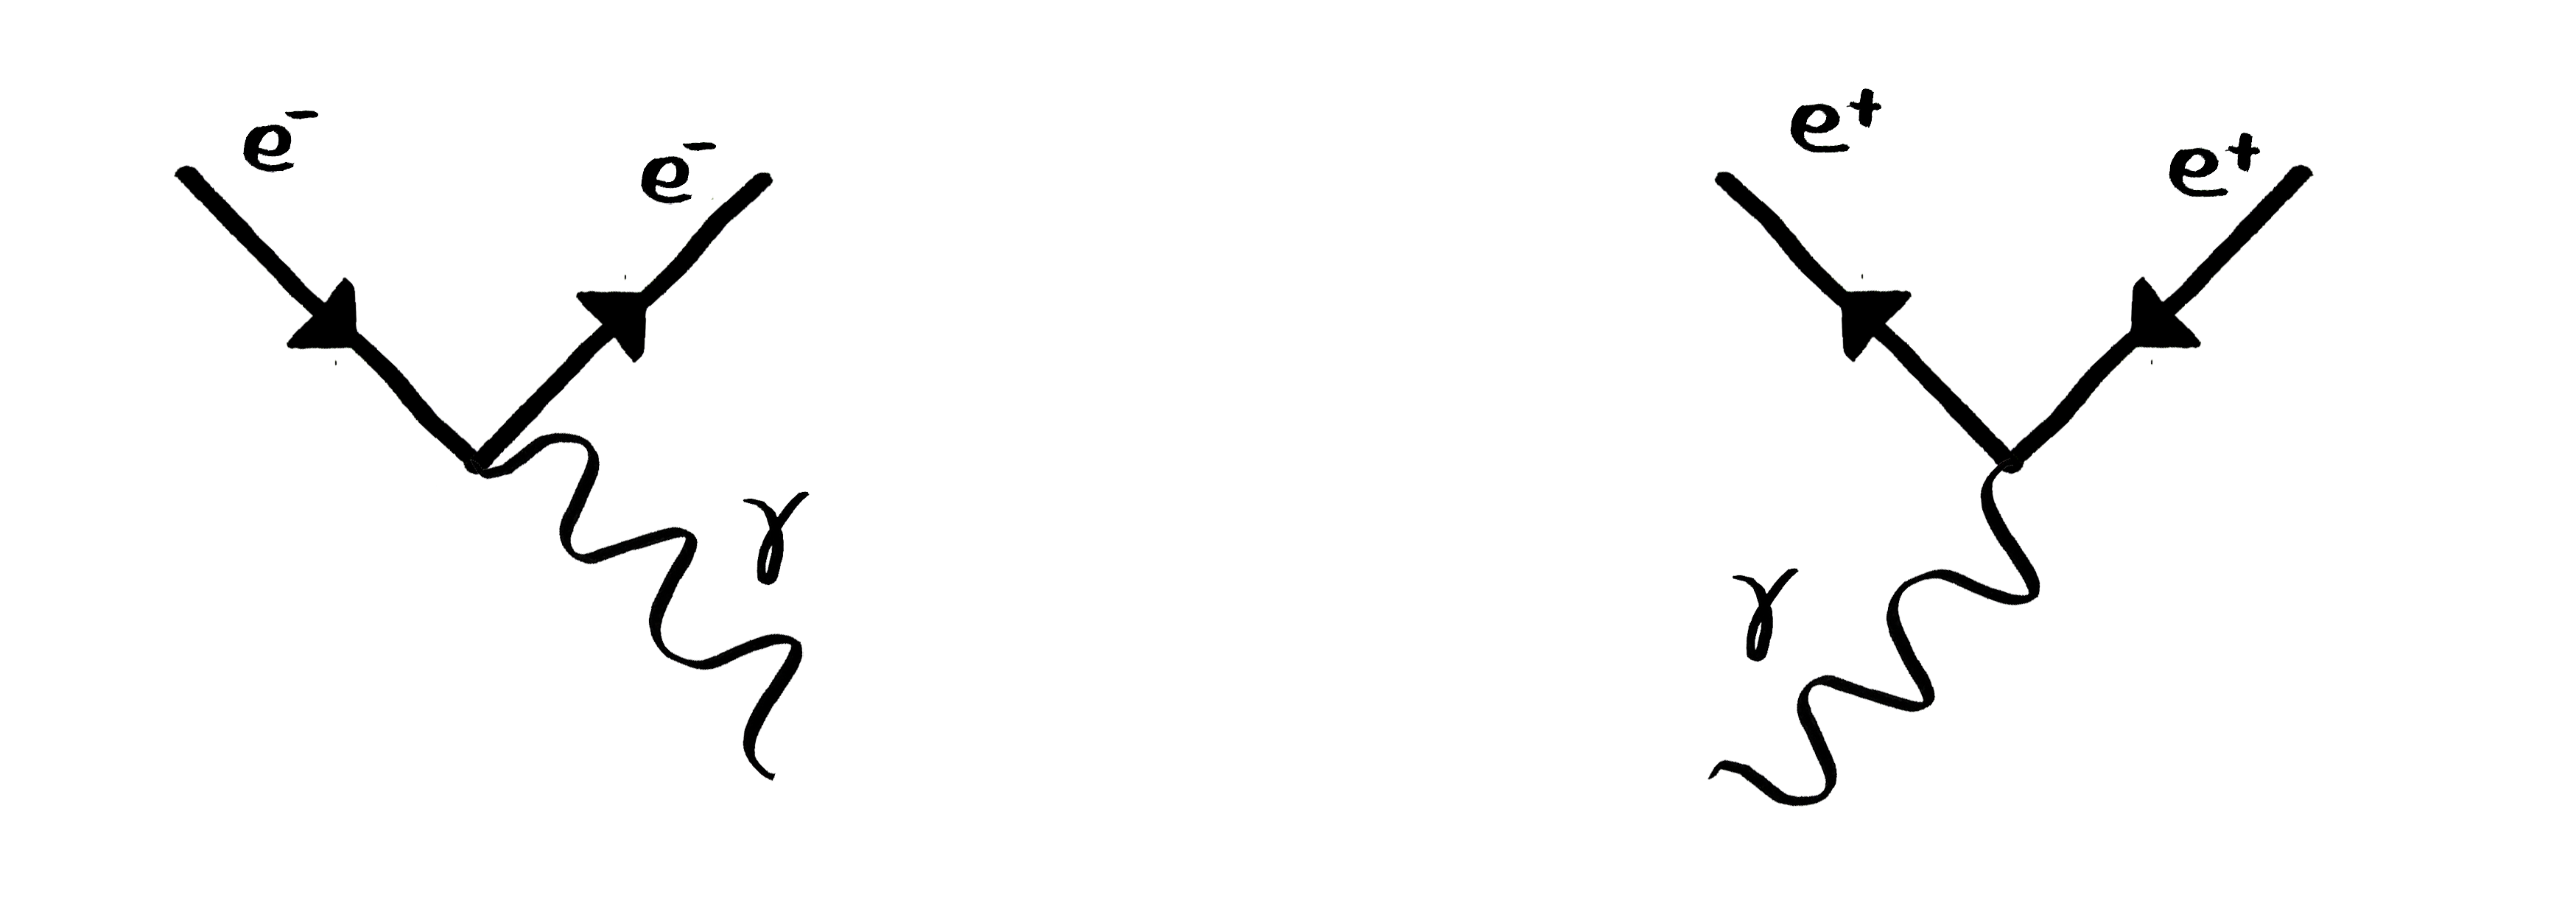
\includegraphics[width=0.6\textwidth]{KernePartikel/fig_p/case_1and22.png}
  \caption{ Venstre: elektron udsender foton. Højre: positron
      absorberer en foton.}
  \label{fig:case_1and2}
\end{figure}
Figur \ref{fig:case_1and2} illustrerer to forskellige scenarier. I
situationen til venstre udsender en elektron en foton og forsætter. I
situationen til højre absorberer en positron en foton og
fortsætter. Kan du overbevise dig selv om, at det er det, der ses på
figuren?

To nye situationer er vist i Figur \ref{fig:case_3and4}. I diagrammet
til venstre annihilerer en elektron og en positron, hvilket skaber en
foton. I diagrammet til højre sker en ''par--dannelse'': en foton
bliver til en elektron og en positron.
\begin{figure}[h!]
  \centering
  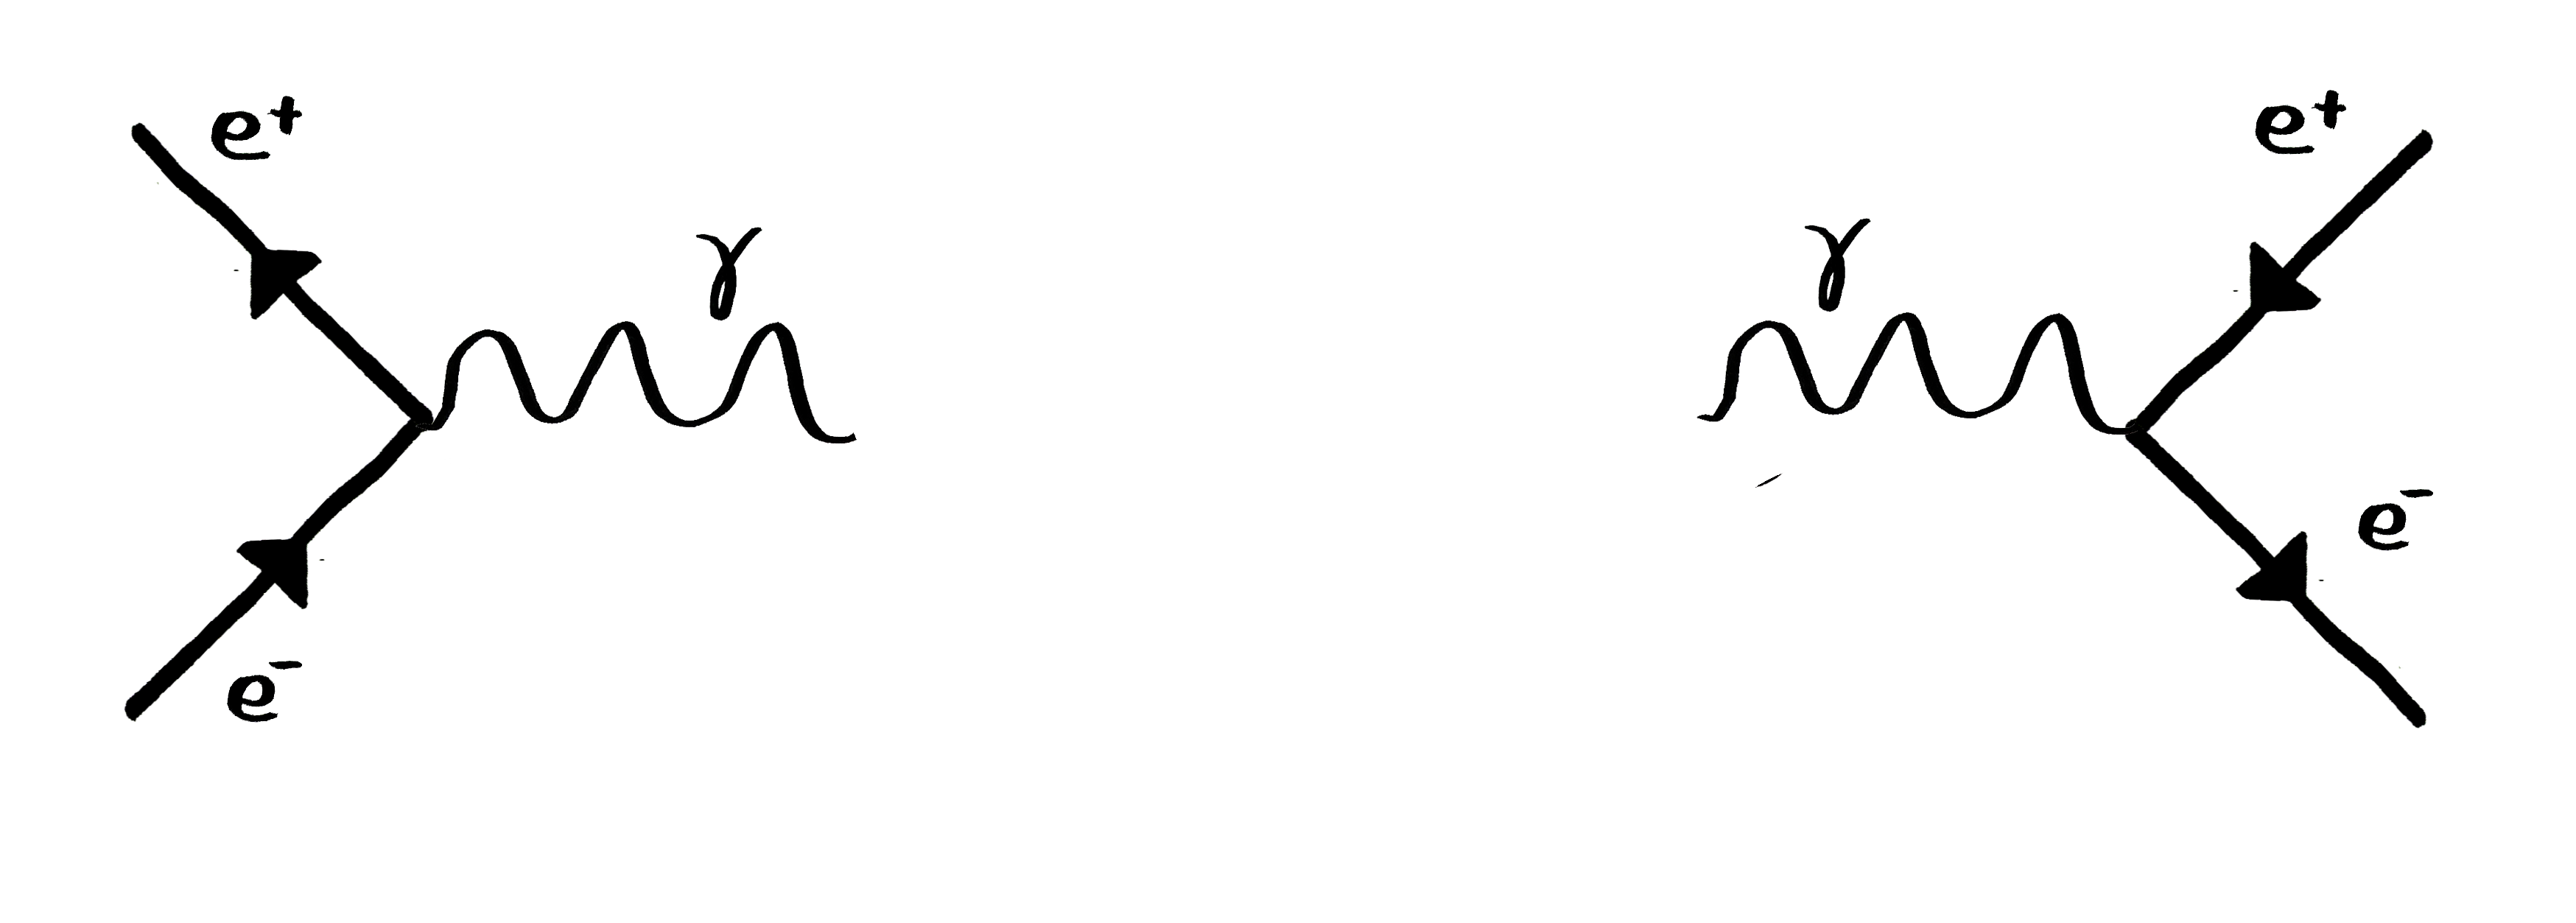
\includegraphics[width=0.6\textwidth]{KernePartikel/fig_p/case_3and42.png}
  \caption{ Venstre: Elektron/positron annihilation. Højre: En
      par-dannelsesproces.}
  \label{fig:case_3and4}
\end{figure}
De fire viste feynman--diagrammer i figur \ref{fig:case_1and2} og
\ref{fig:case_3and4} indeholder alle de samme elementer, men hvordan de
er orienteret i diagrammet gør alligevel en stor forskel for den
fysiske betydning!  

En anden vigtig force ved feynman--diagrammer er, at de kan roteres. Når en partikel under en rotation af et feynman--diagram passerer grænsen mellem venstre side (de indgående partikler) og den højre side (de udgående partikler) skifter den til sin anti-partikel. Det er utroligt brugbart at feynman--diagrammer der fungerer i én orientering, også fungerer når diagrammet er roteret, så længe man husker at skifte partiklerne ud med deres antipartikler, når de passerer grænsen mellem indgående og udgående partikler.

Vi husker på, at det, der befinder sig på venstre
side af feynman--diagrammet er de indkommende partikler -- de partikler
som enten skal kollidere med hinanden, eller som skal til at lave noget
interessant fysik, og de partikler, som ses til højre i diagrammet er
de udgående partikler -- de partikler man ville måle i sin
partikelaccelerator. Pas på med ikke at tolke retningen på pilene som
den retning, partiklerne rejser -- pilenes retning angiver udelukkende
om der er tale om en partikel eller en anti--partikel.

\subsubsection{Reaktioner med $W^{\pm}$-partiklen}

$W$--partiklen er en af de bosoner, som bærer den svage vekselvirkning. De er f.eks. tilstede i reaktioner, hvor der enten udsendes eller absorberes neutrionoer. Dens ladning, som enten kan være +1 eller -1, skrevet som hhv. $W^+$ og $W^-$ kommer an på ladningen af partiklerne i reaktionen. 

\begin{figure}[h!]
  \centering
  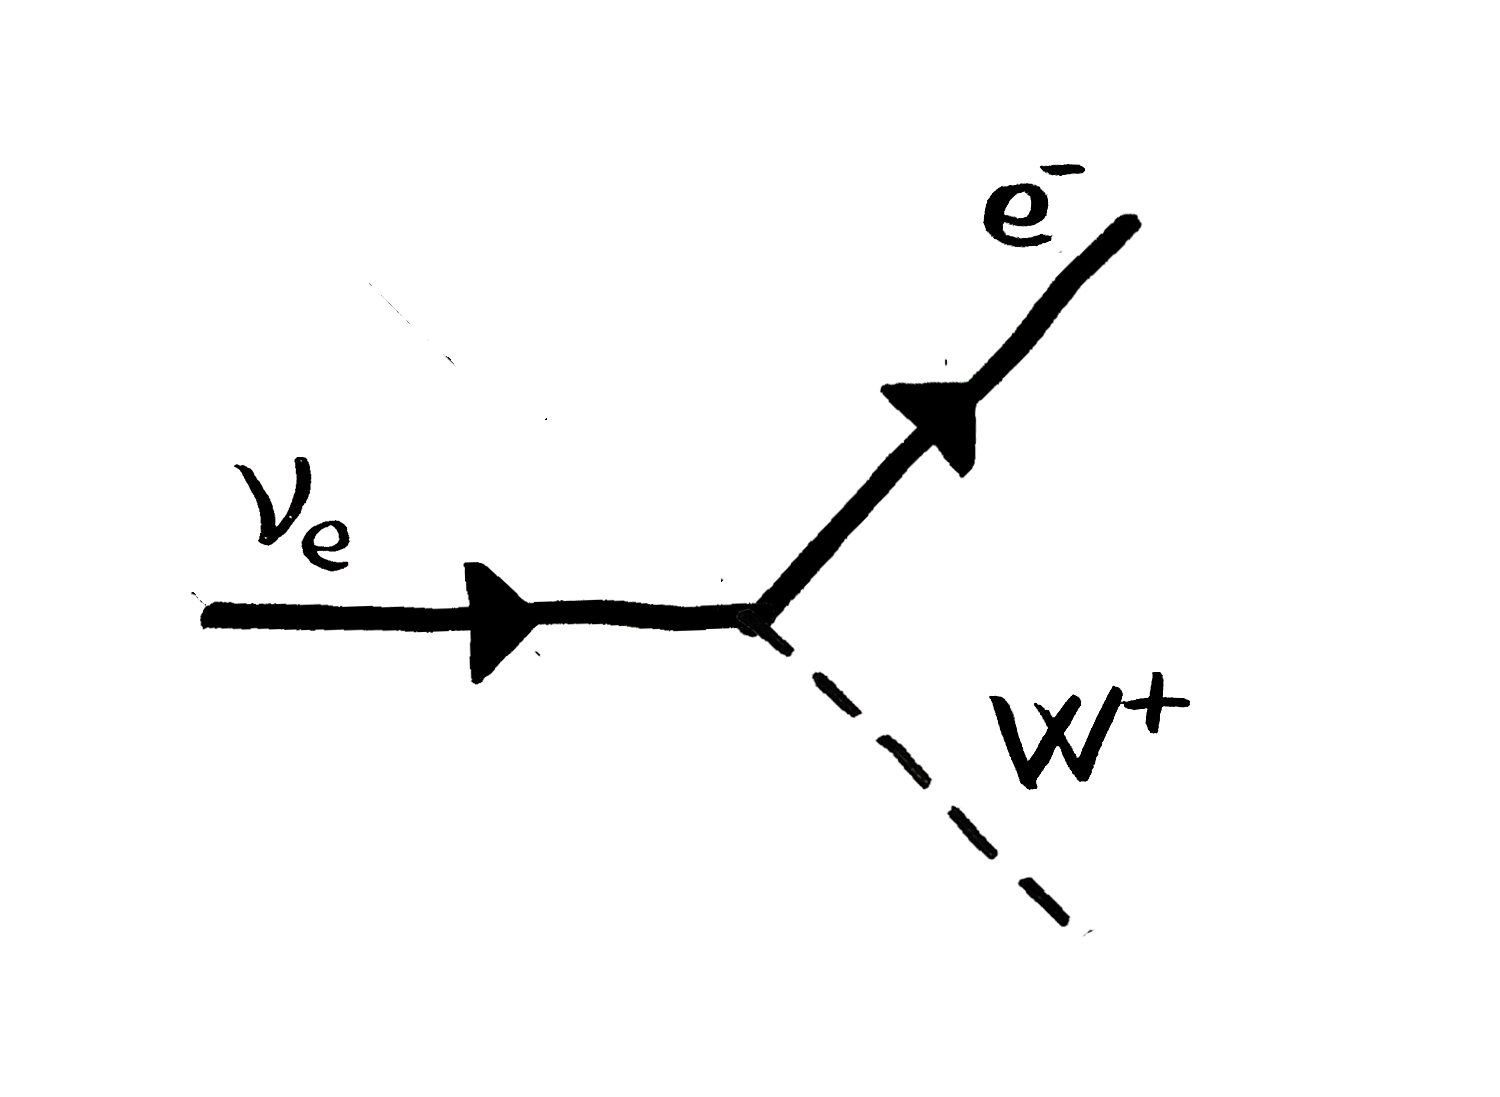
\includegraphics[width=0.3\textwidth]{KernePartikel/fig_p/weak_vertex.png}
  \caption{ Udsendelse af en $W^+$-boson.}
  \label{fig:weak_vertex}
\end{figure}

Betragt reaktionen i Figur \ref{fig:weak_vertex}.
Det viser omdannelsen af en elektron--neutrino til en elektron under udsendelse af en $W$--partikel. For at opnå ladningsbevarelse i reaktionen må ladningen af $W$ være +1. For at skelne melem de forskellige typer vekselvirkninger er det normalt at bosoner fra den svage vekselvirkning tegnes som en stiplet streg, som det ses på figuren. 

$W$--partiklen kendes bedst for sin rolle i kernehenfald, som f.eks. i tilfældet med beta--minus--henfald. Her er reaktionen som bekendt at en neutron henfalder til en proton, elektron og antineutrino:
\begin{equation}
n \rightarrow p + e^- + \bar{\nu}_e.
\end{equation}
Men $W$-bosonen er til stede i denne raktion en som virtuel partikel. Faktisk udsender neutronen under sin omdannelse til en proton en $W$--partikel, som efterfølgende henfalder til en elektron og en antineutrino. Feynman--diagrammet for et beta--minus--henfald er vist i Figur \ref{fig:beta_minus}. Det ses at $W$--bosonen er en virtuel partikel, idet den eksisterer mellem to vertexer. 

\begin{figure}[h!]
  \centering
  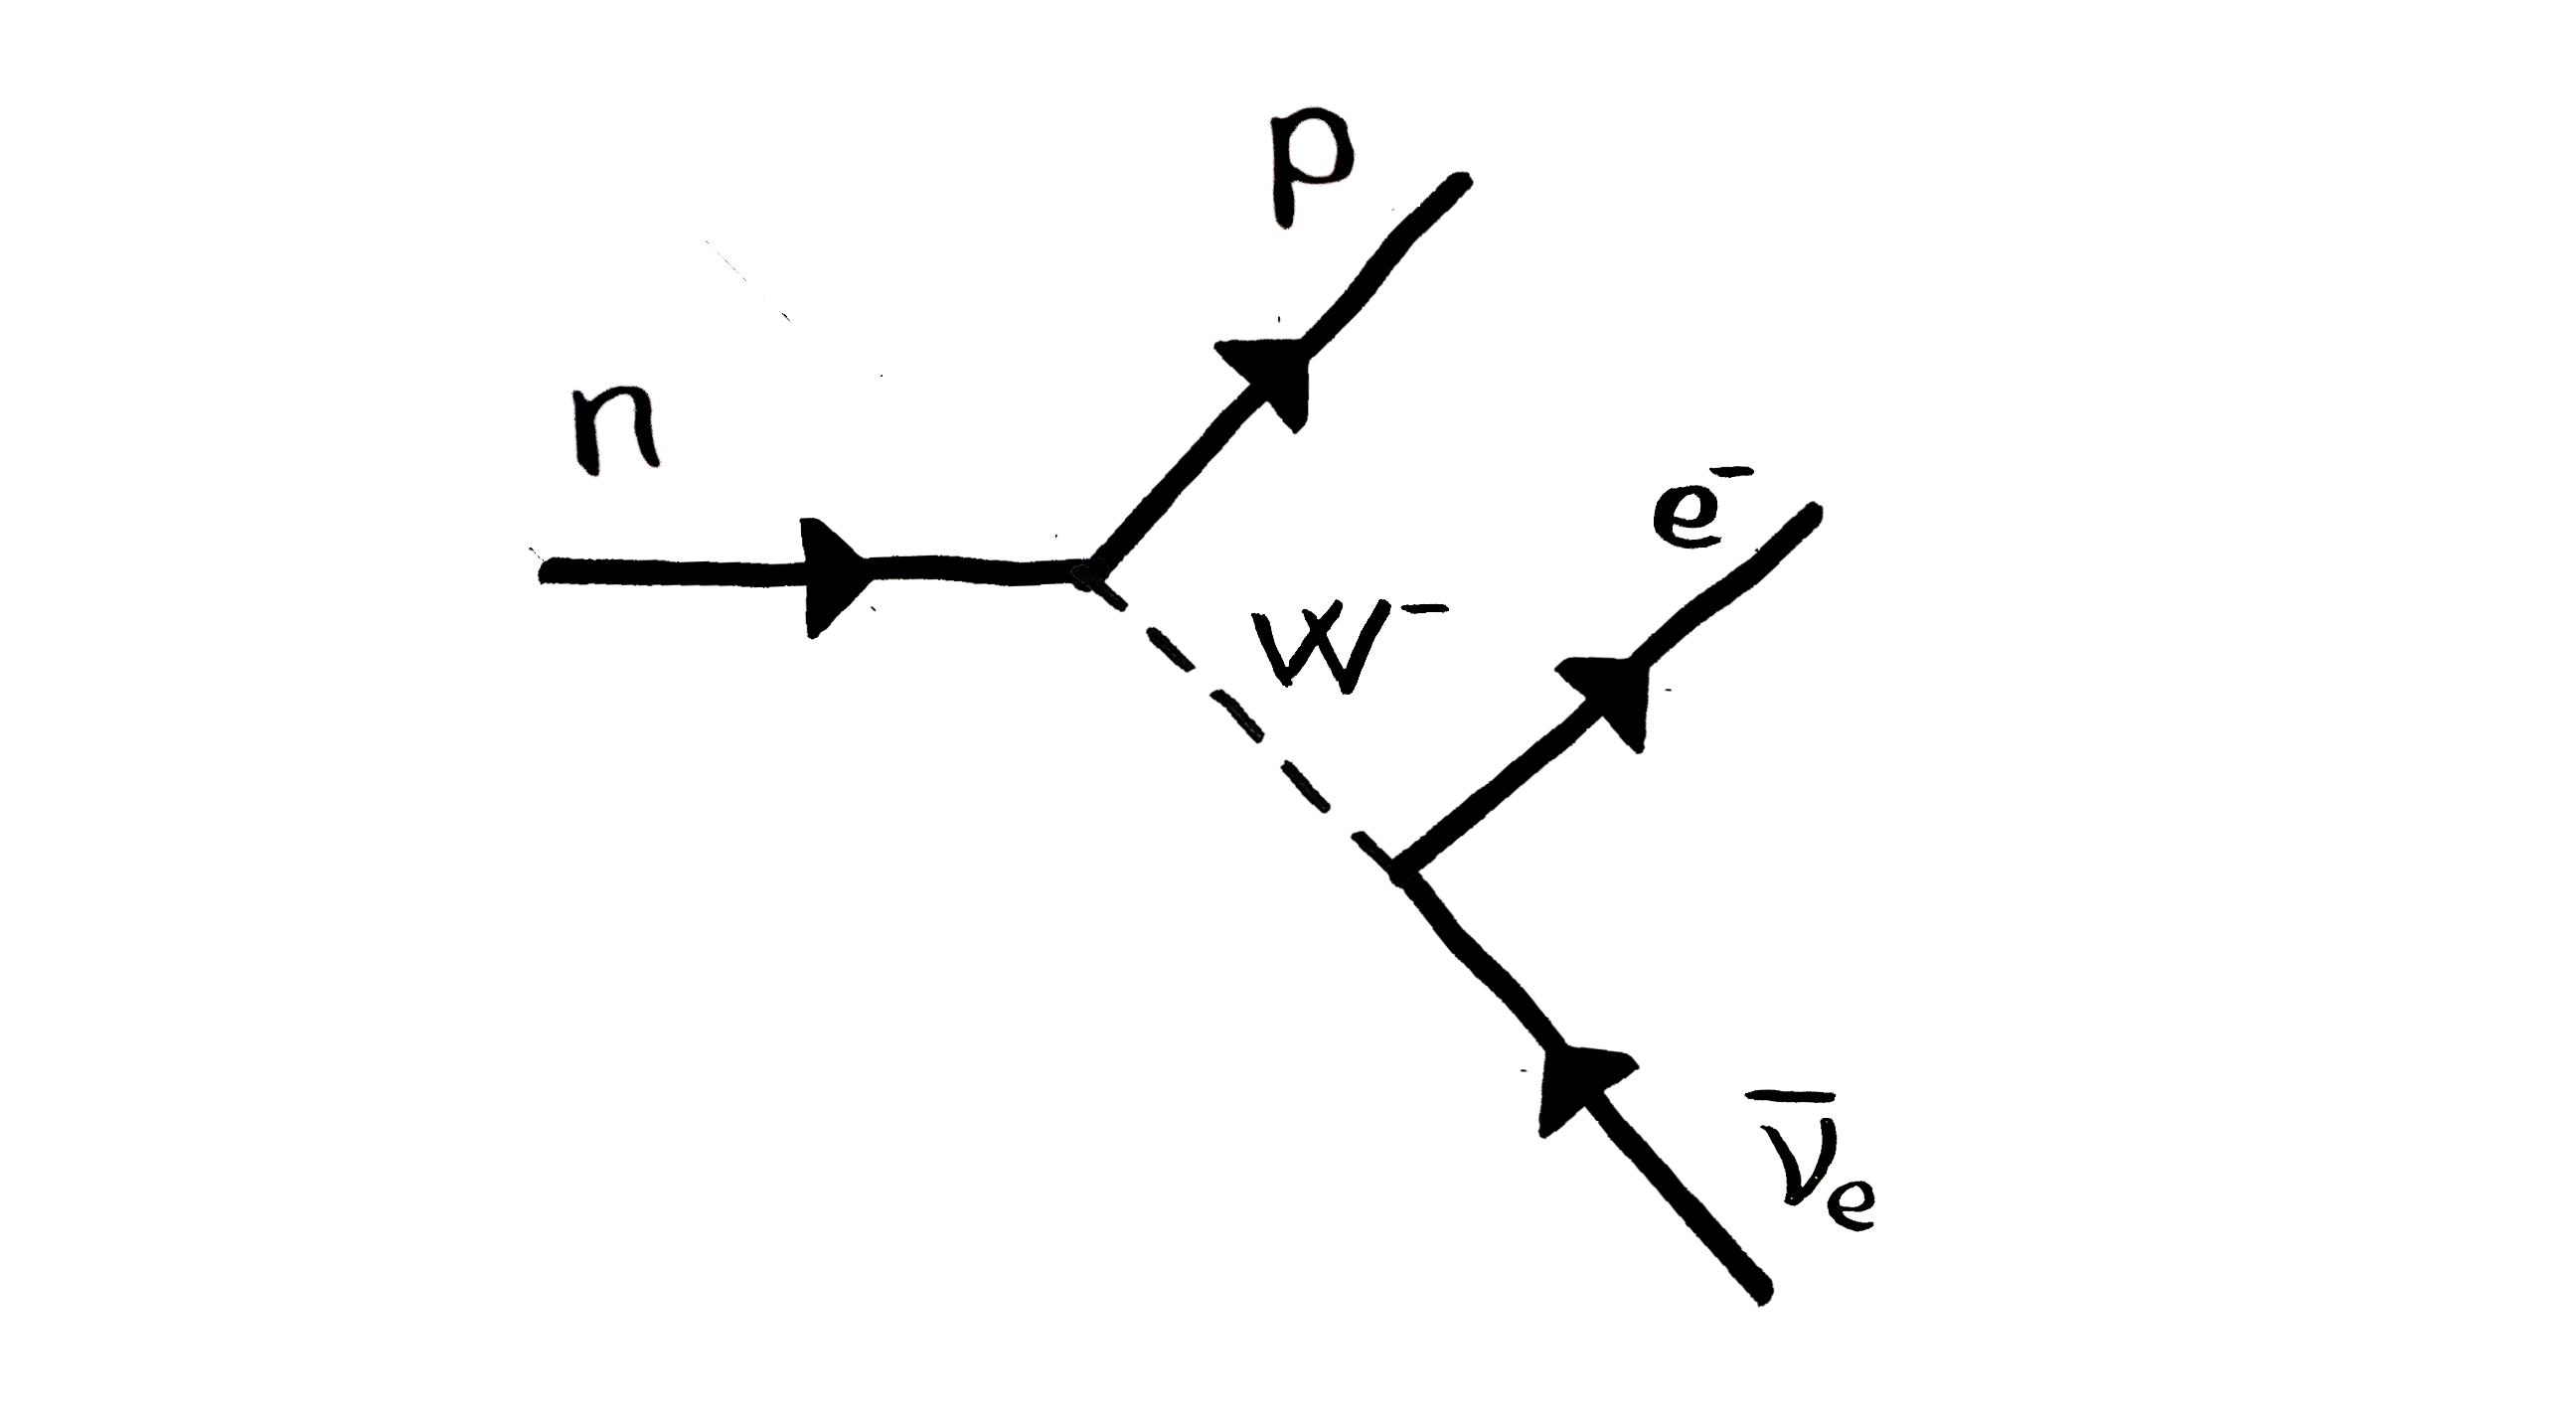
\includegraphics[width=0.4\textwidth]{KernePartikel/fig_p/beta_minus.png}
  \caption{ Beta-minus-henfald}
  \label{fig:beta_minus}
\end{figure}

Vi husker på, at neutronen og protonen ikke er elementære partikler, men faktisk består af kvarker. $W$--bosonen kan ændre kvarker af bestemt en type, kaldet smage (\emph{eng:flavour}). Kvarkerne kan omdannes ved hjælp af $W$--boson således at de ændrer deres ladning med enten $\pm1$, f.eks. u$\leftrightarrow$d. 

